\documentclass[a4paper]{article}
\usepackage{placeins}
\usepackage{graphics}
\usepackage[dvipsnames]{xcolor}
\usepackage{natbib}
\usepackage{graphicx}
\usepackage{placeins}
\usepackage{float}
\usepackage{url}
\usepackage{subfig}
\usepackage{hyperref}

\hypersetup{
  colorlinks=true,
  linkcolor=Blue,
  citecolor=Blue,
  filecolor=magenta,      
  urlcolor=cyan,
 }


\begin{document}

\title{Supplementary : data analysis methods}

\tableofcontents

\section{Cell type annotation}

\subsection{Scatter plots}

\begin{figure}[!htb]
  \centering
  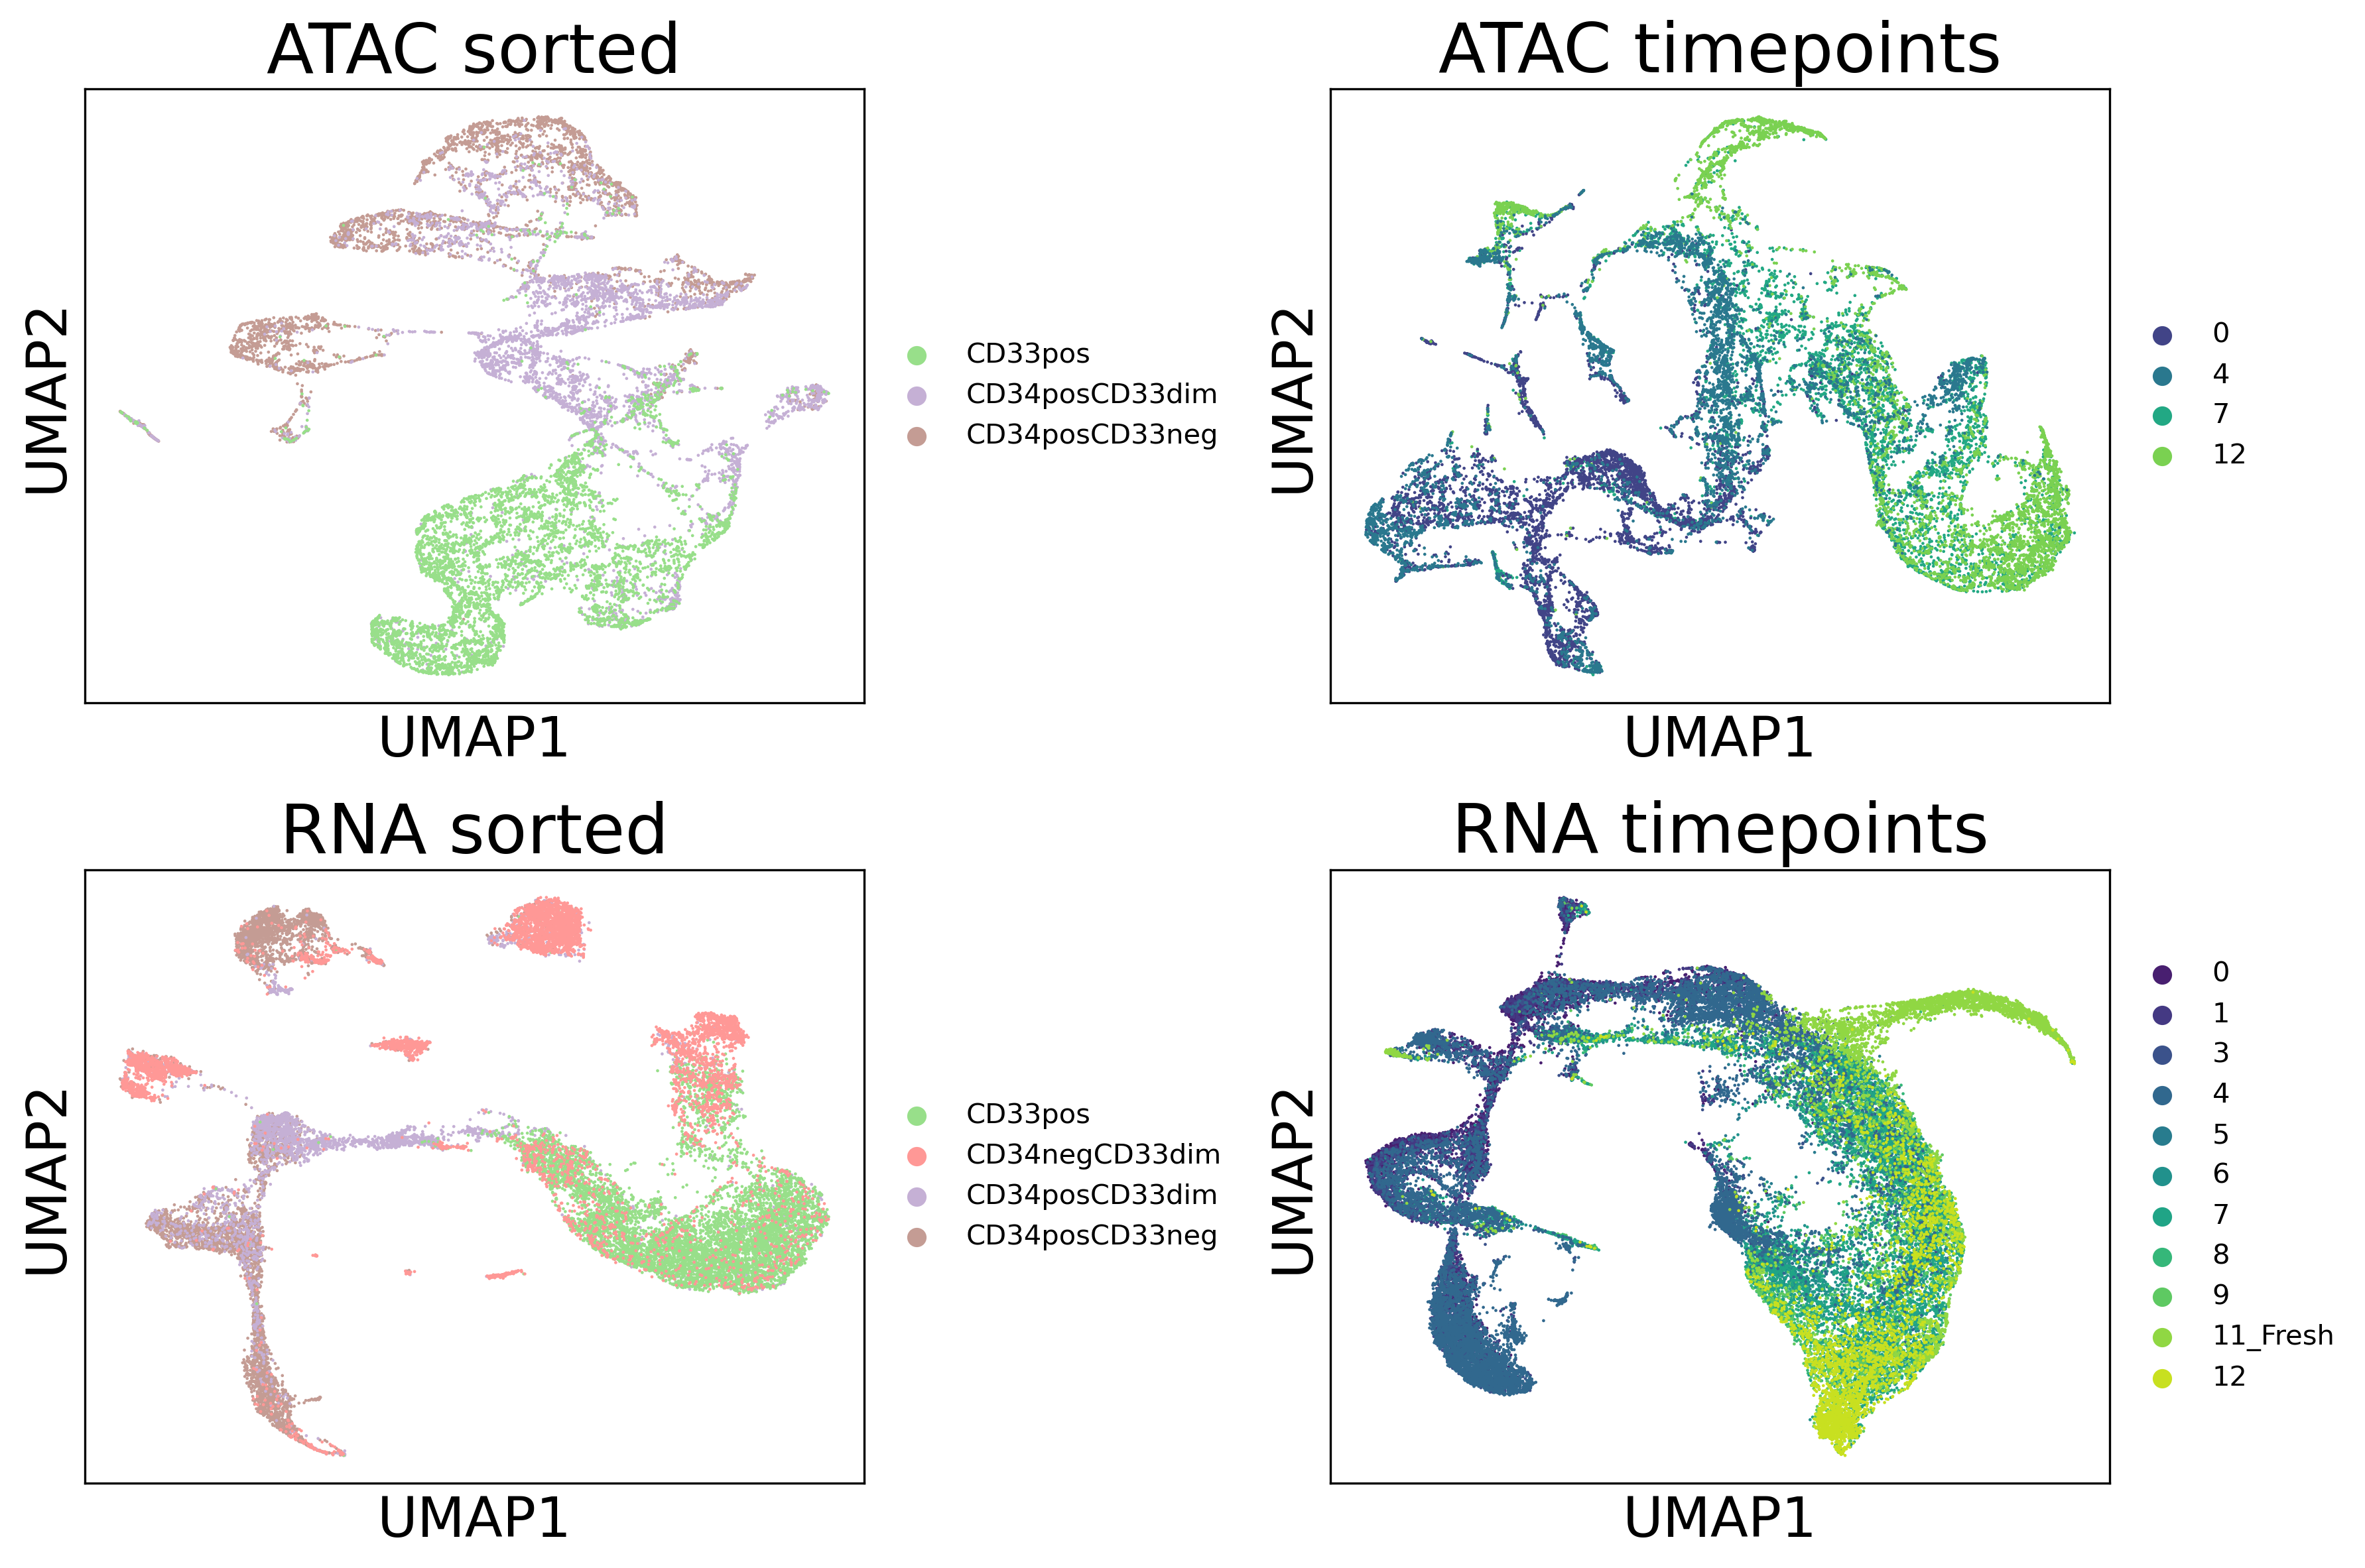
\includegraphics[width=\textwidth]{../figures/hematopoiesis/label.png}
  \caption{Scatter: Time points (days) and sorted assays (CD) annotation}
\end{figure}

\begin{figure}[!htb]
  \centering
  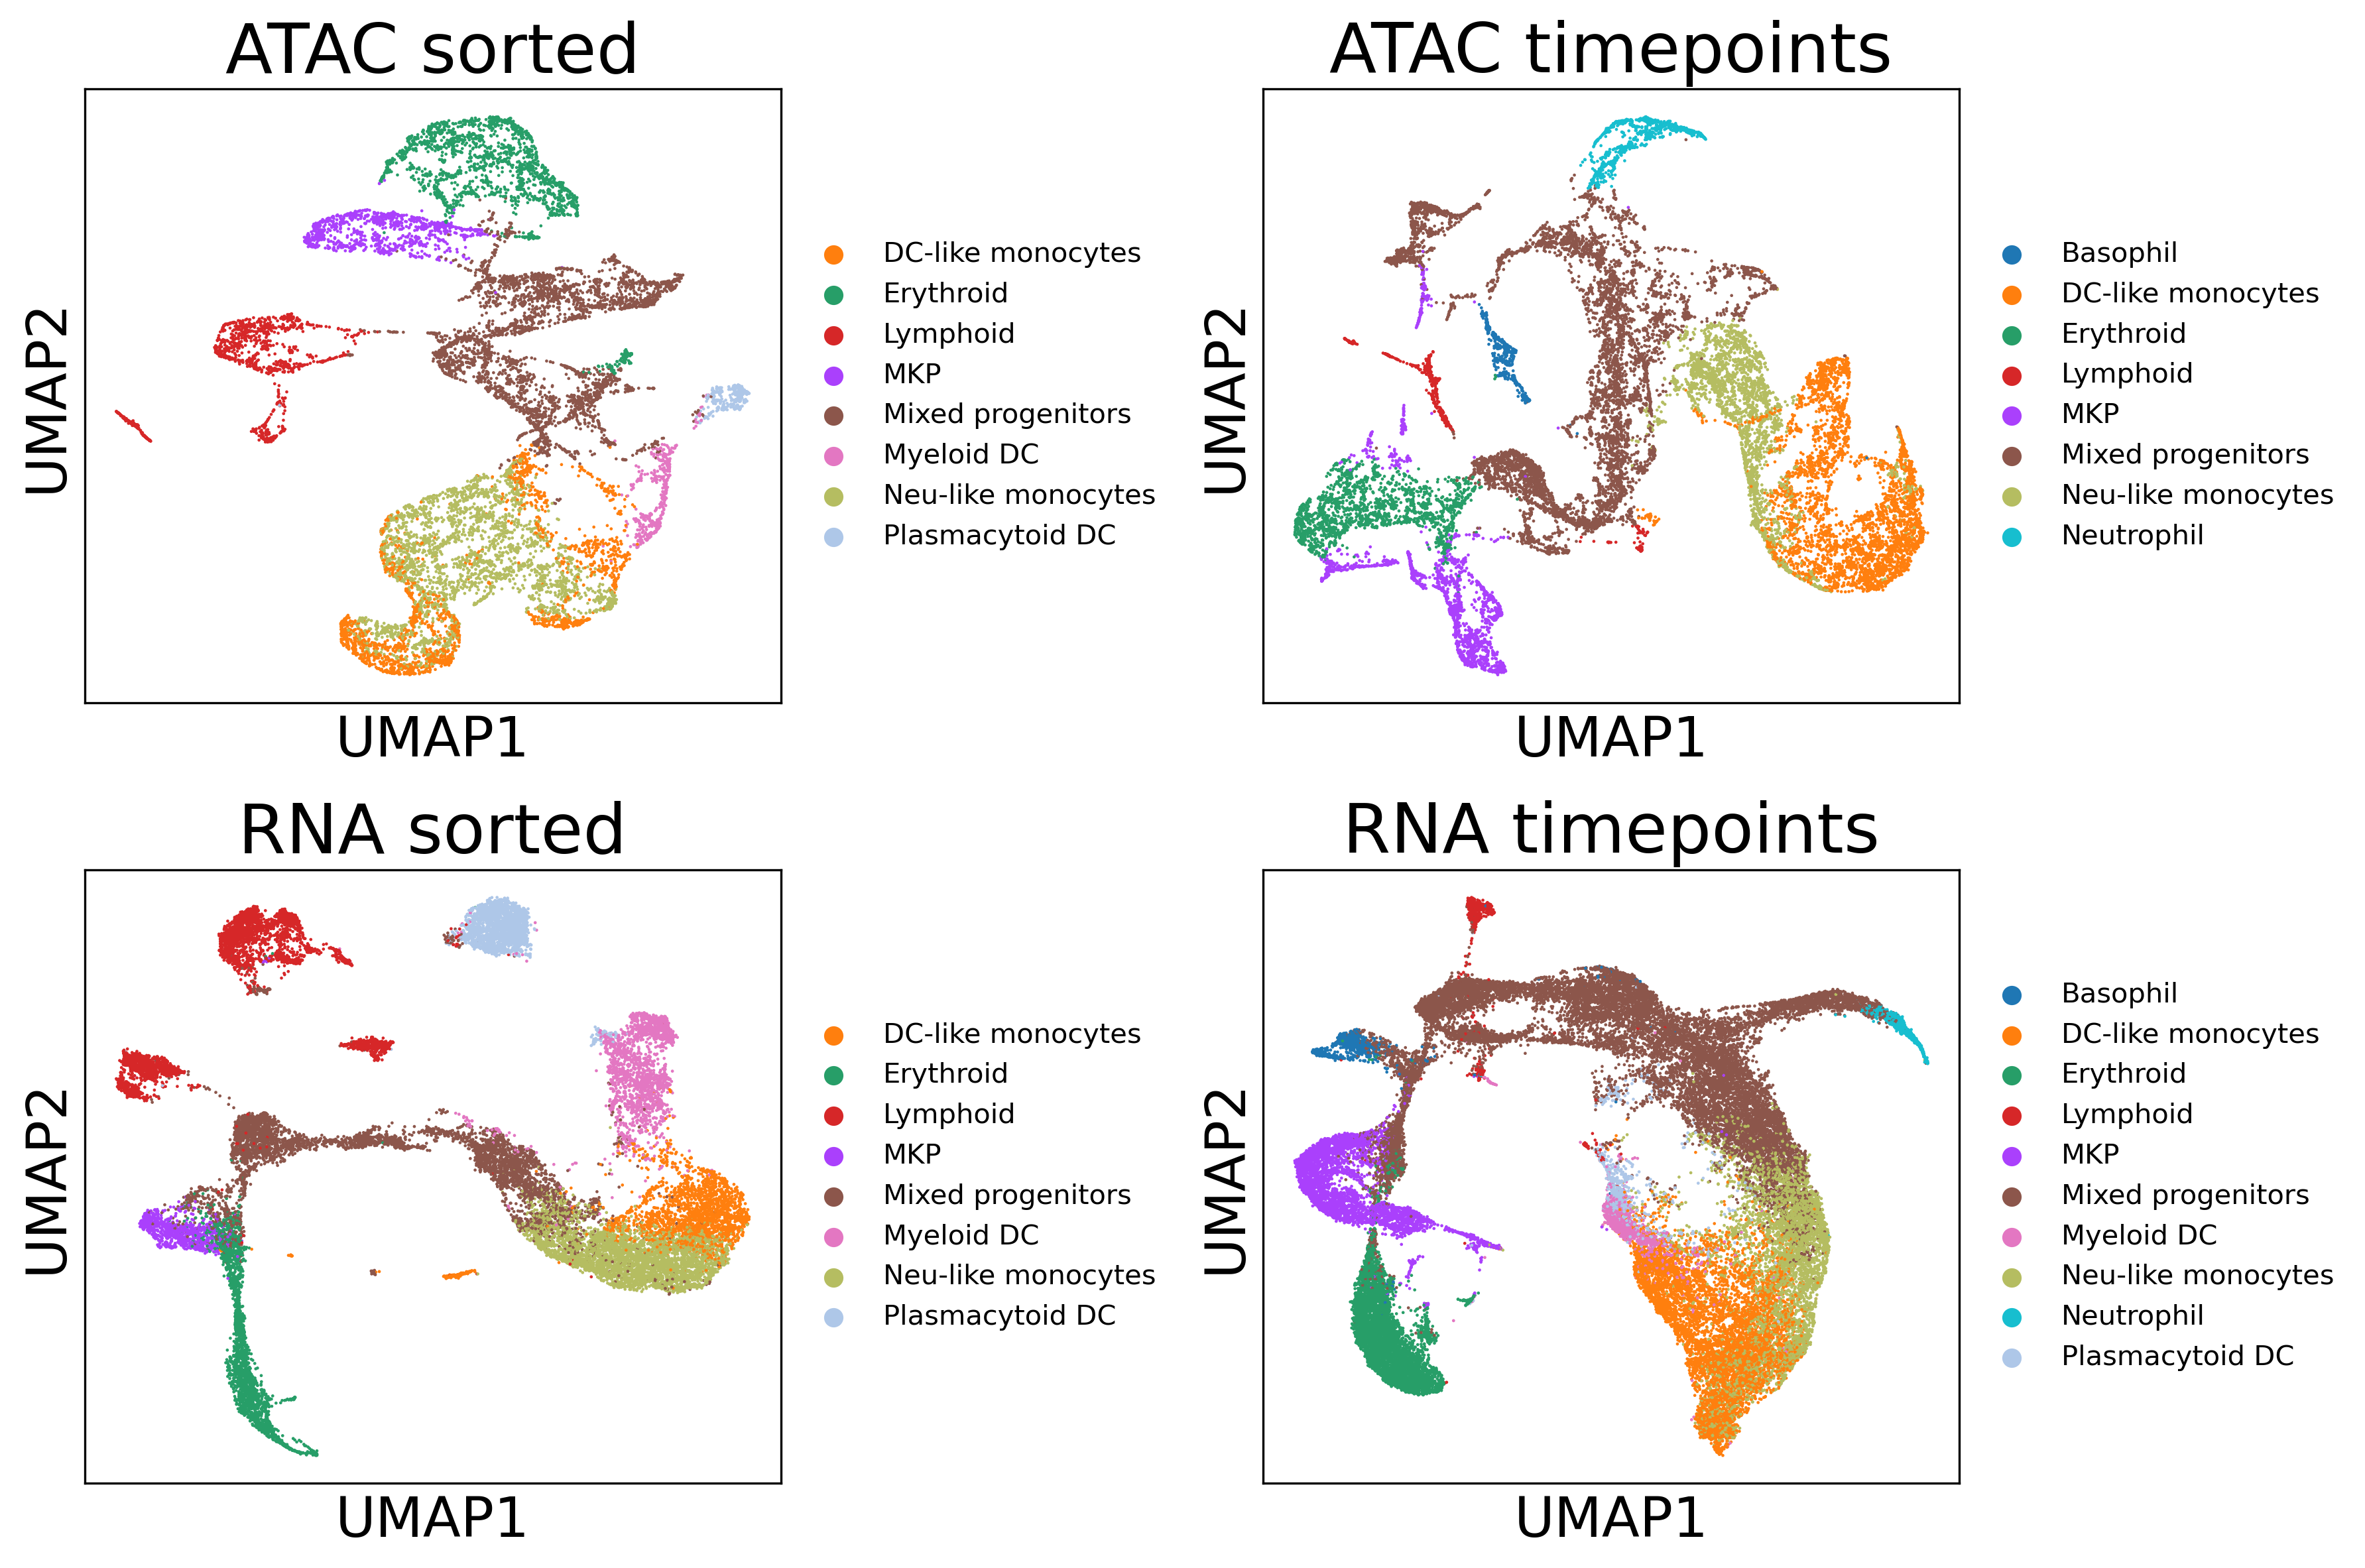
\includegraphics[width=\textwidth]{../figures/hematopoiesis/leiden_identity_simple2.png}
  \caption{Scatter: Leiden identity simple annotation}
\end{figure}

\begin{figure}[!htb]
  \centering
  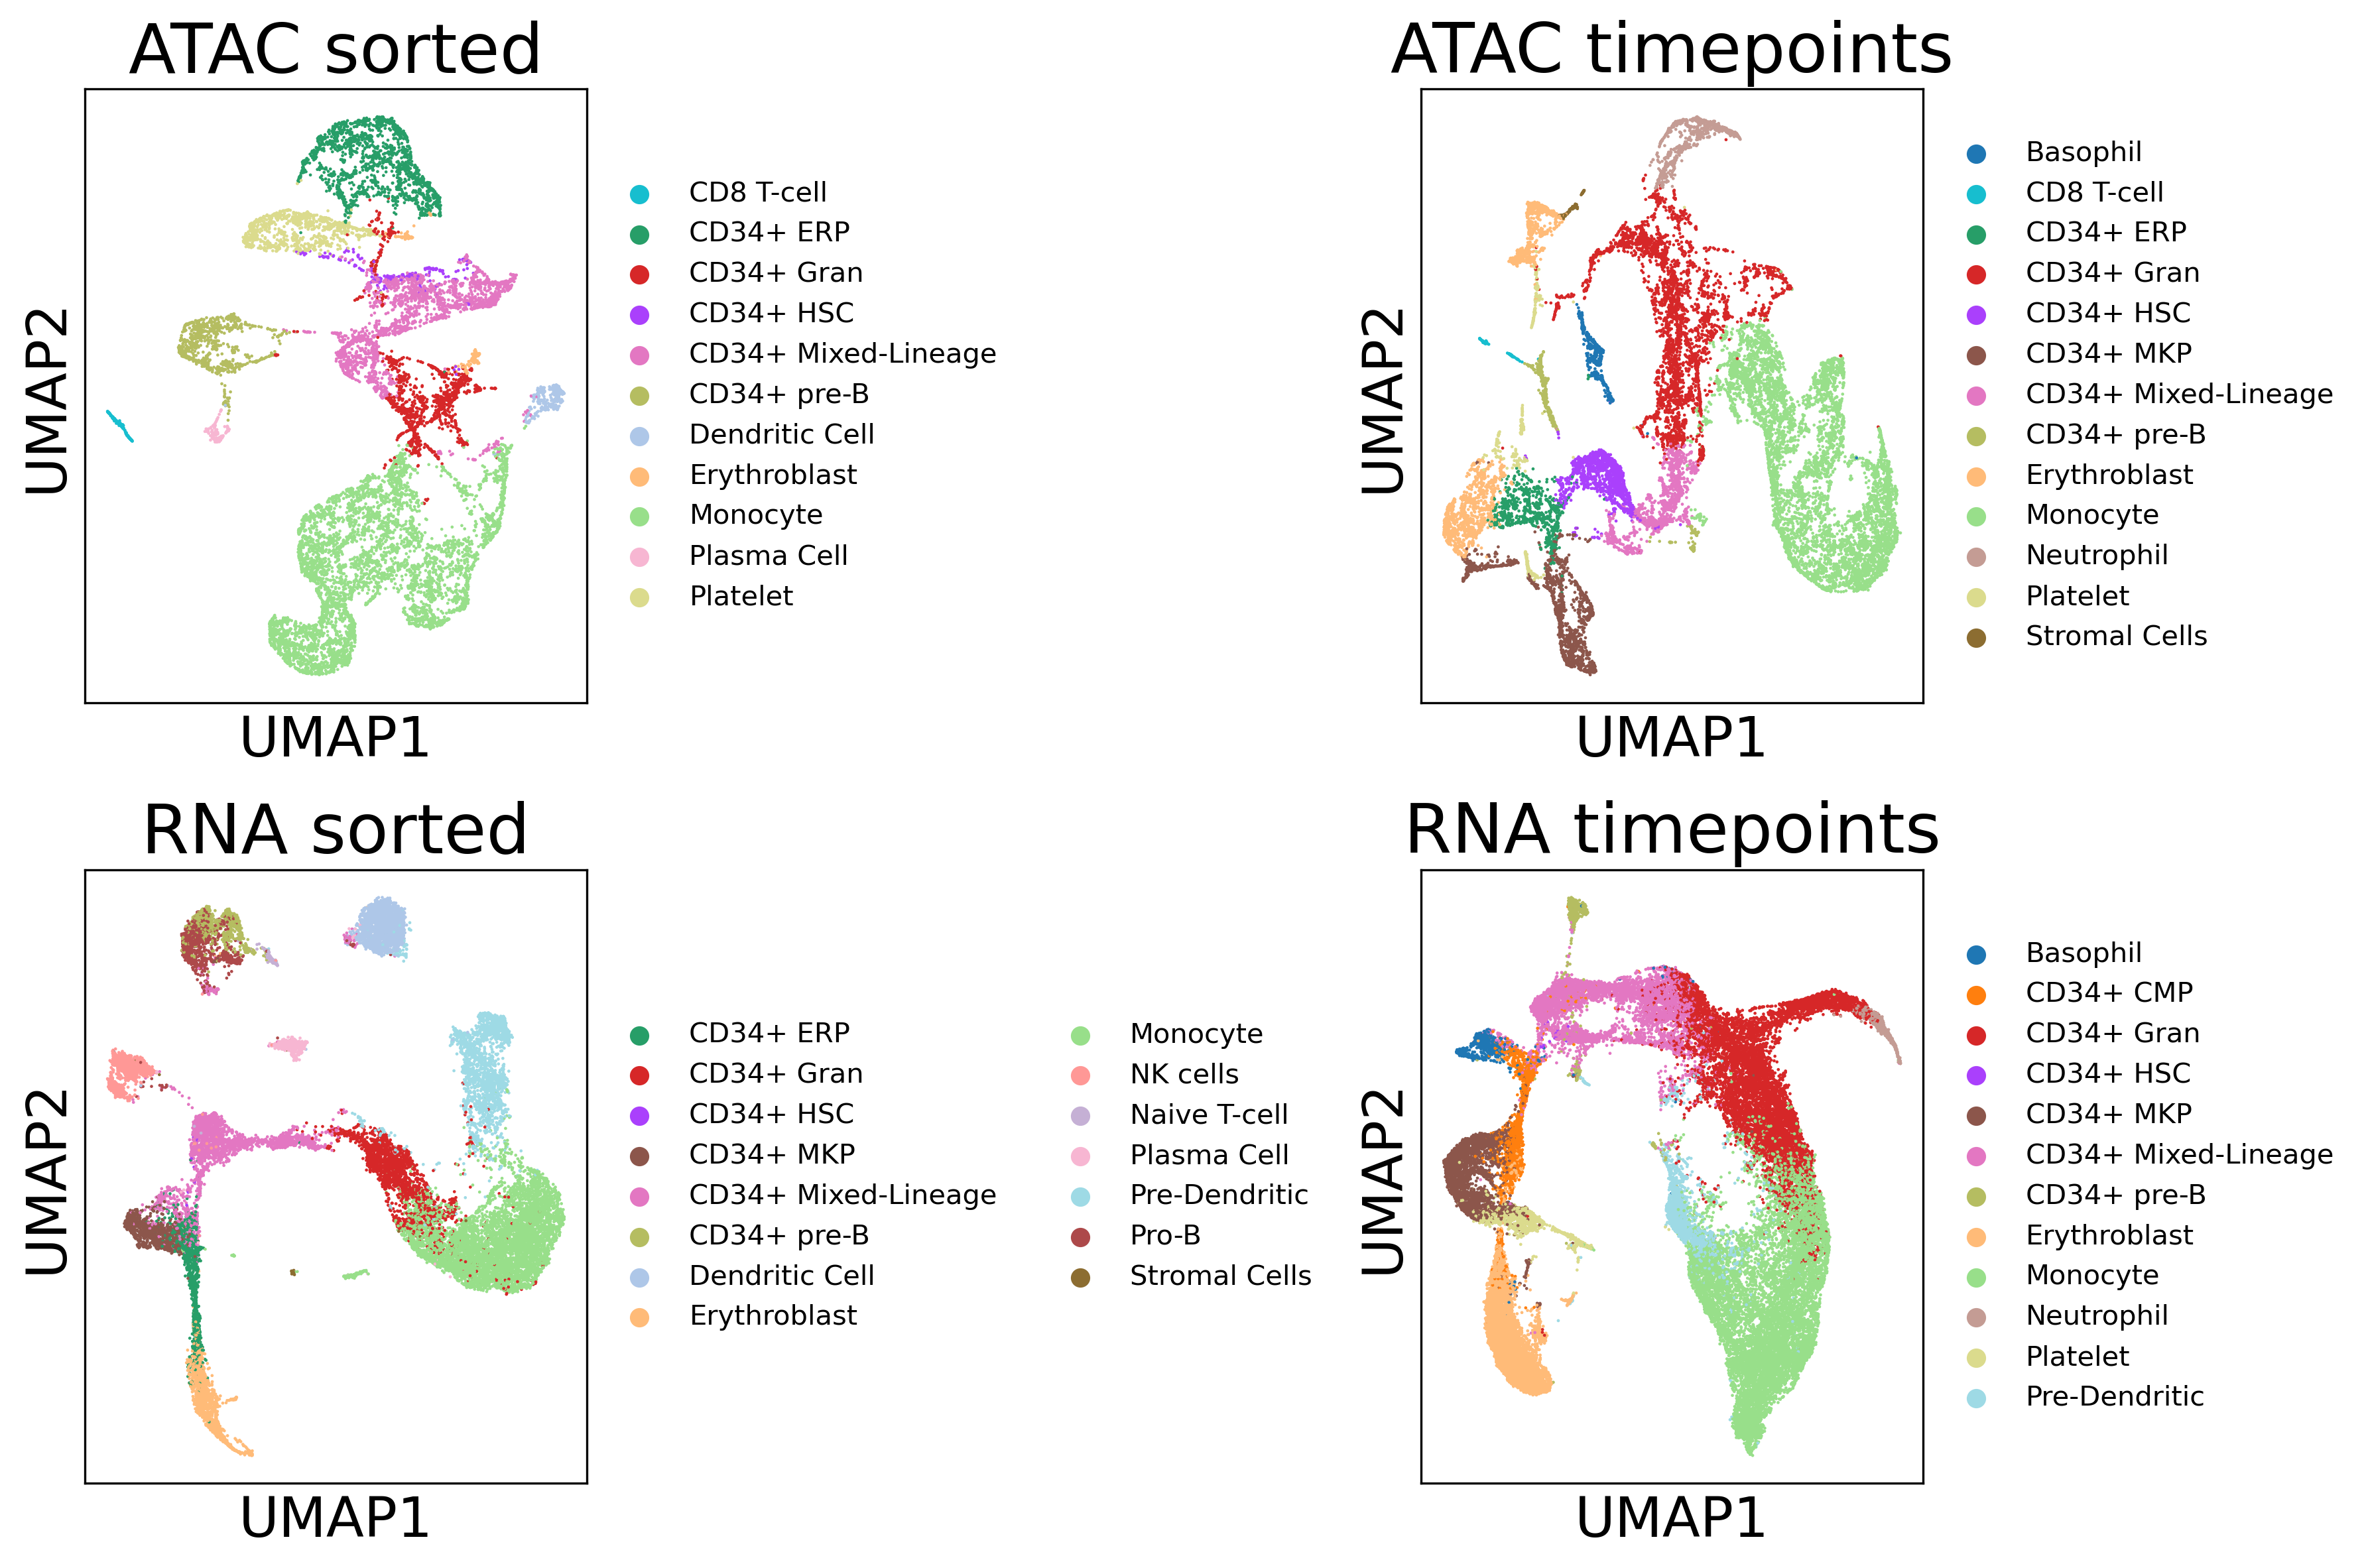
\includegraphics[width=\textwidth]{../figures/hematopoiesis/leiden_identity.png}
  \caption{Scatter: Leiden identity annotation}
\end{figure}

\FloatBarrier
\subsection{Bar plots}

\begin{figure}[!htb]
  \centering
  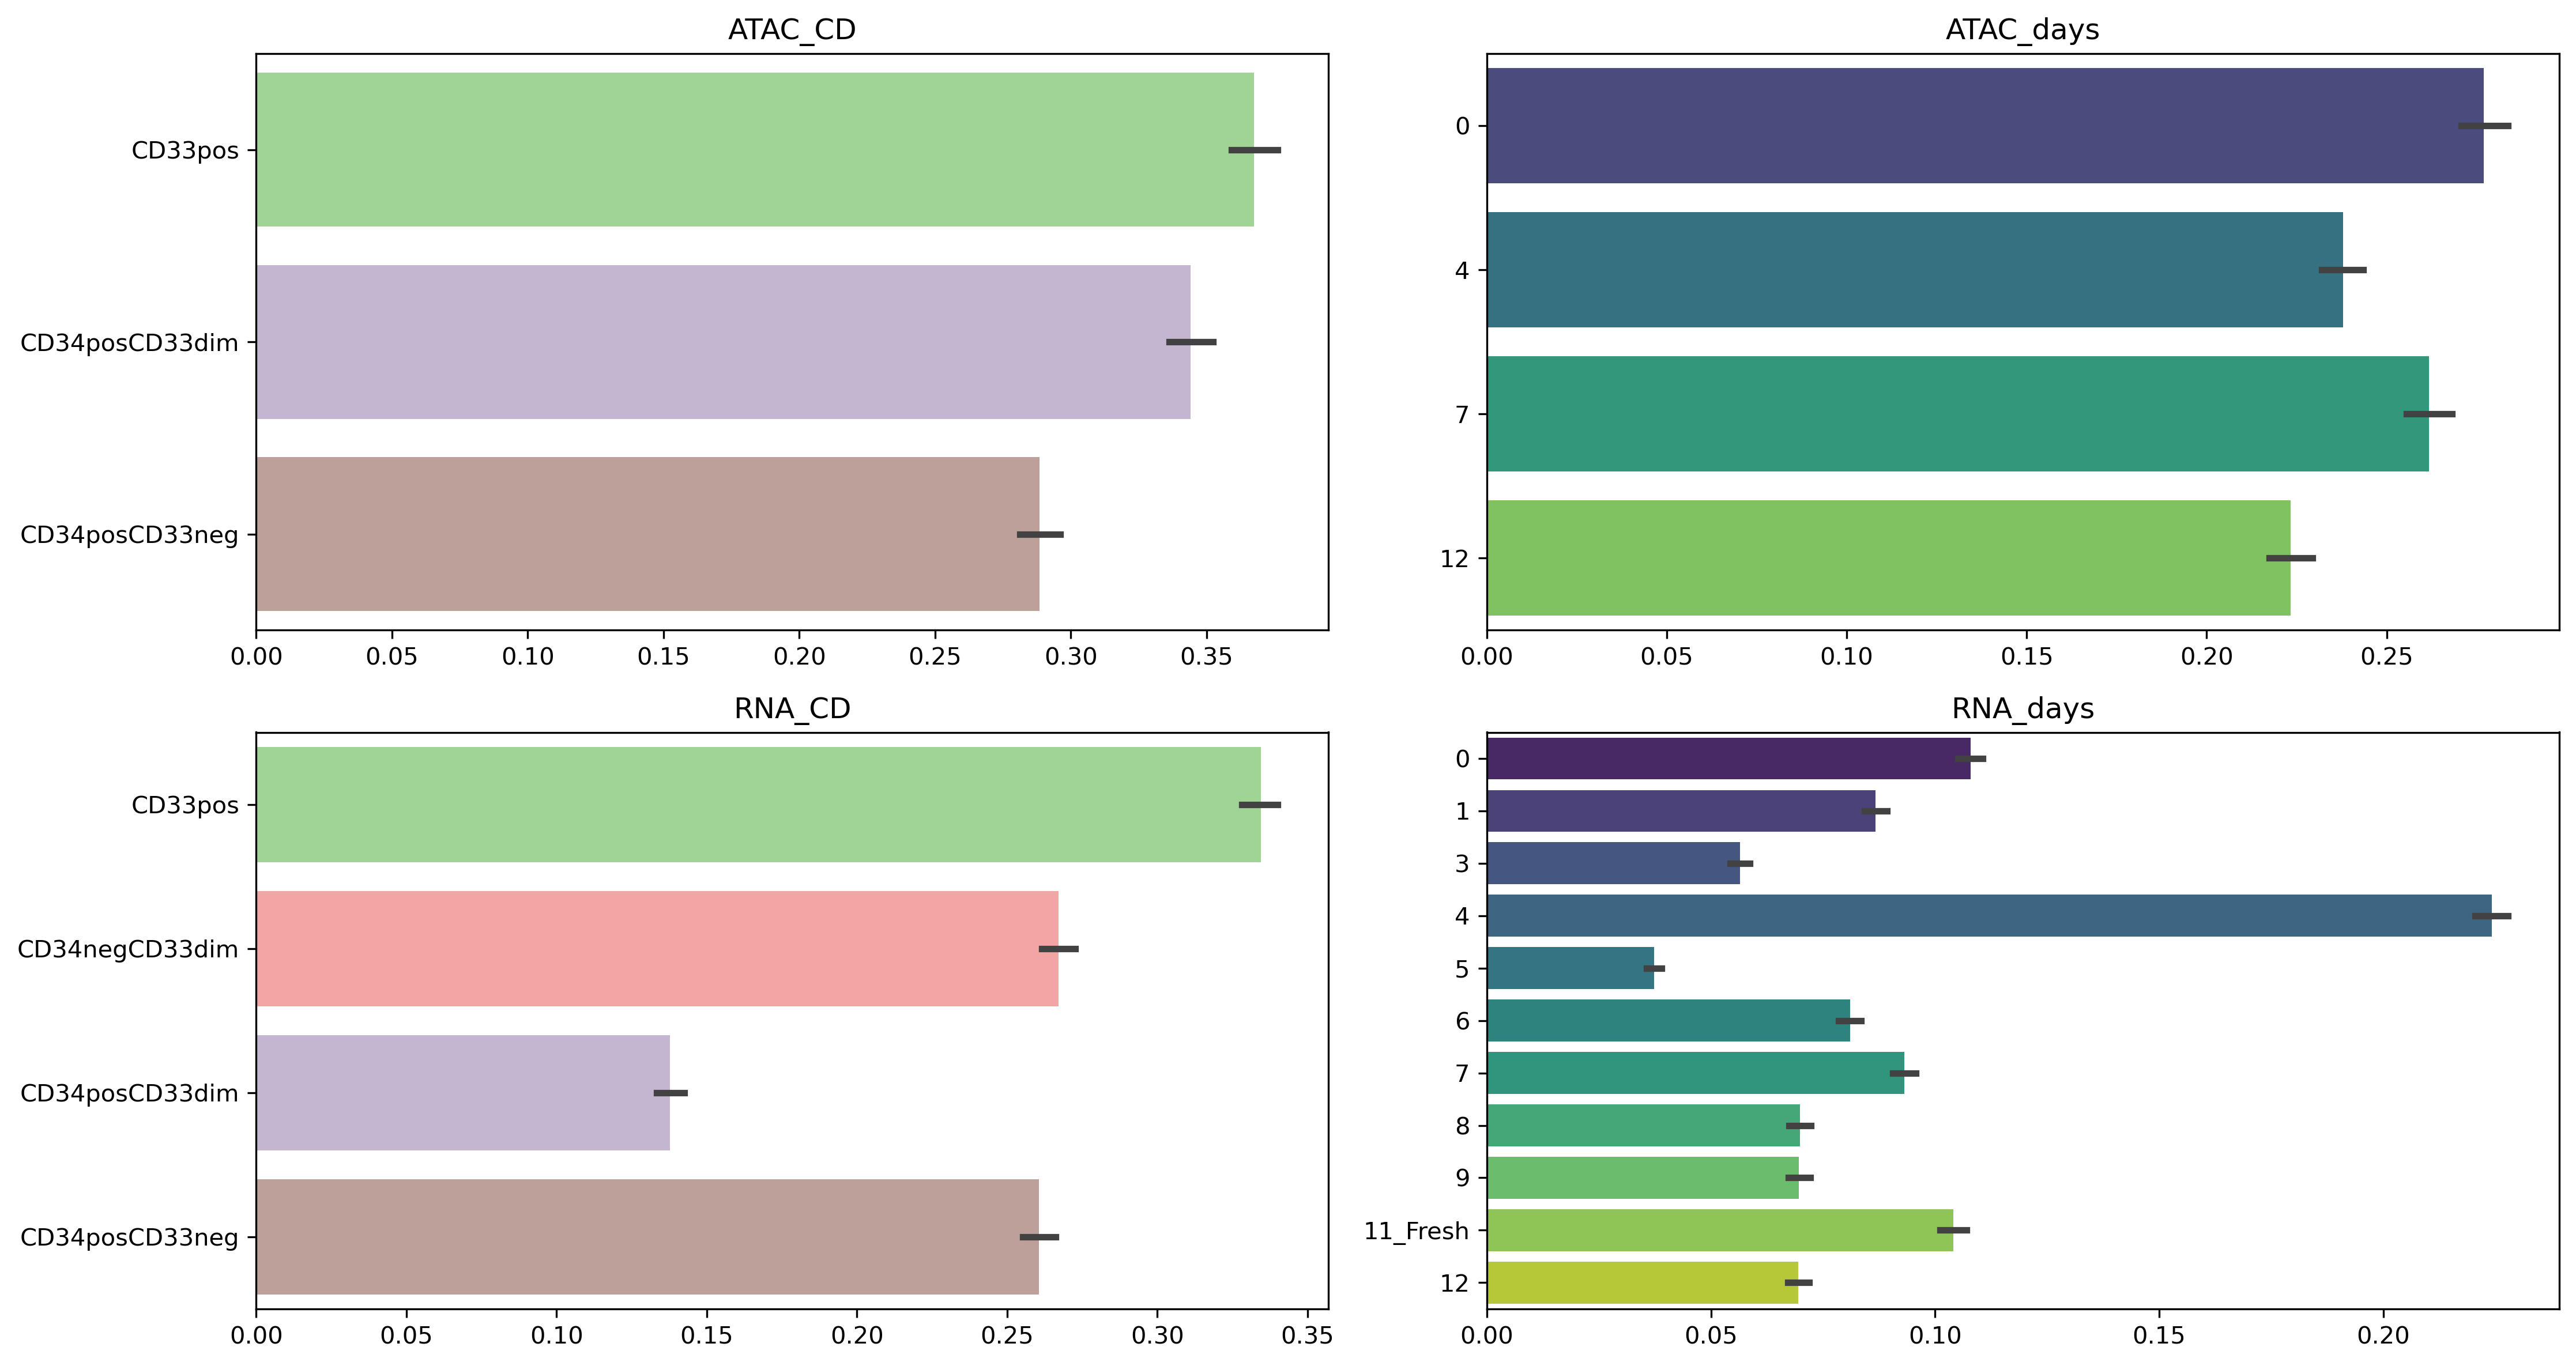
\includegraphics[width=\textwidth]{../figures/hematopoiesis/label_proportions.png}
  \caption{Proportions: Leiden identity simple annotation}
\end{figure}

\begin{figure}[!htb]
  \centering
  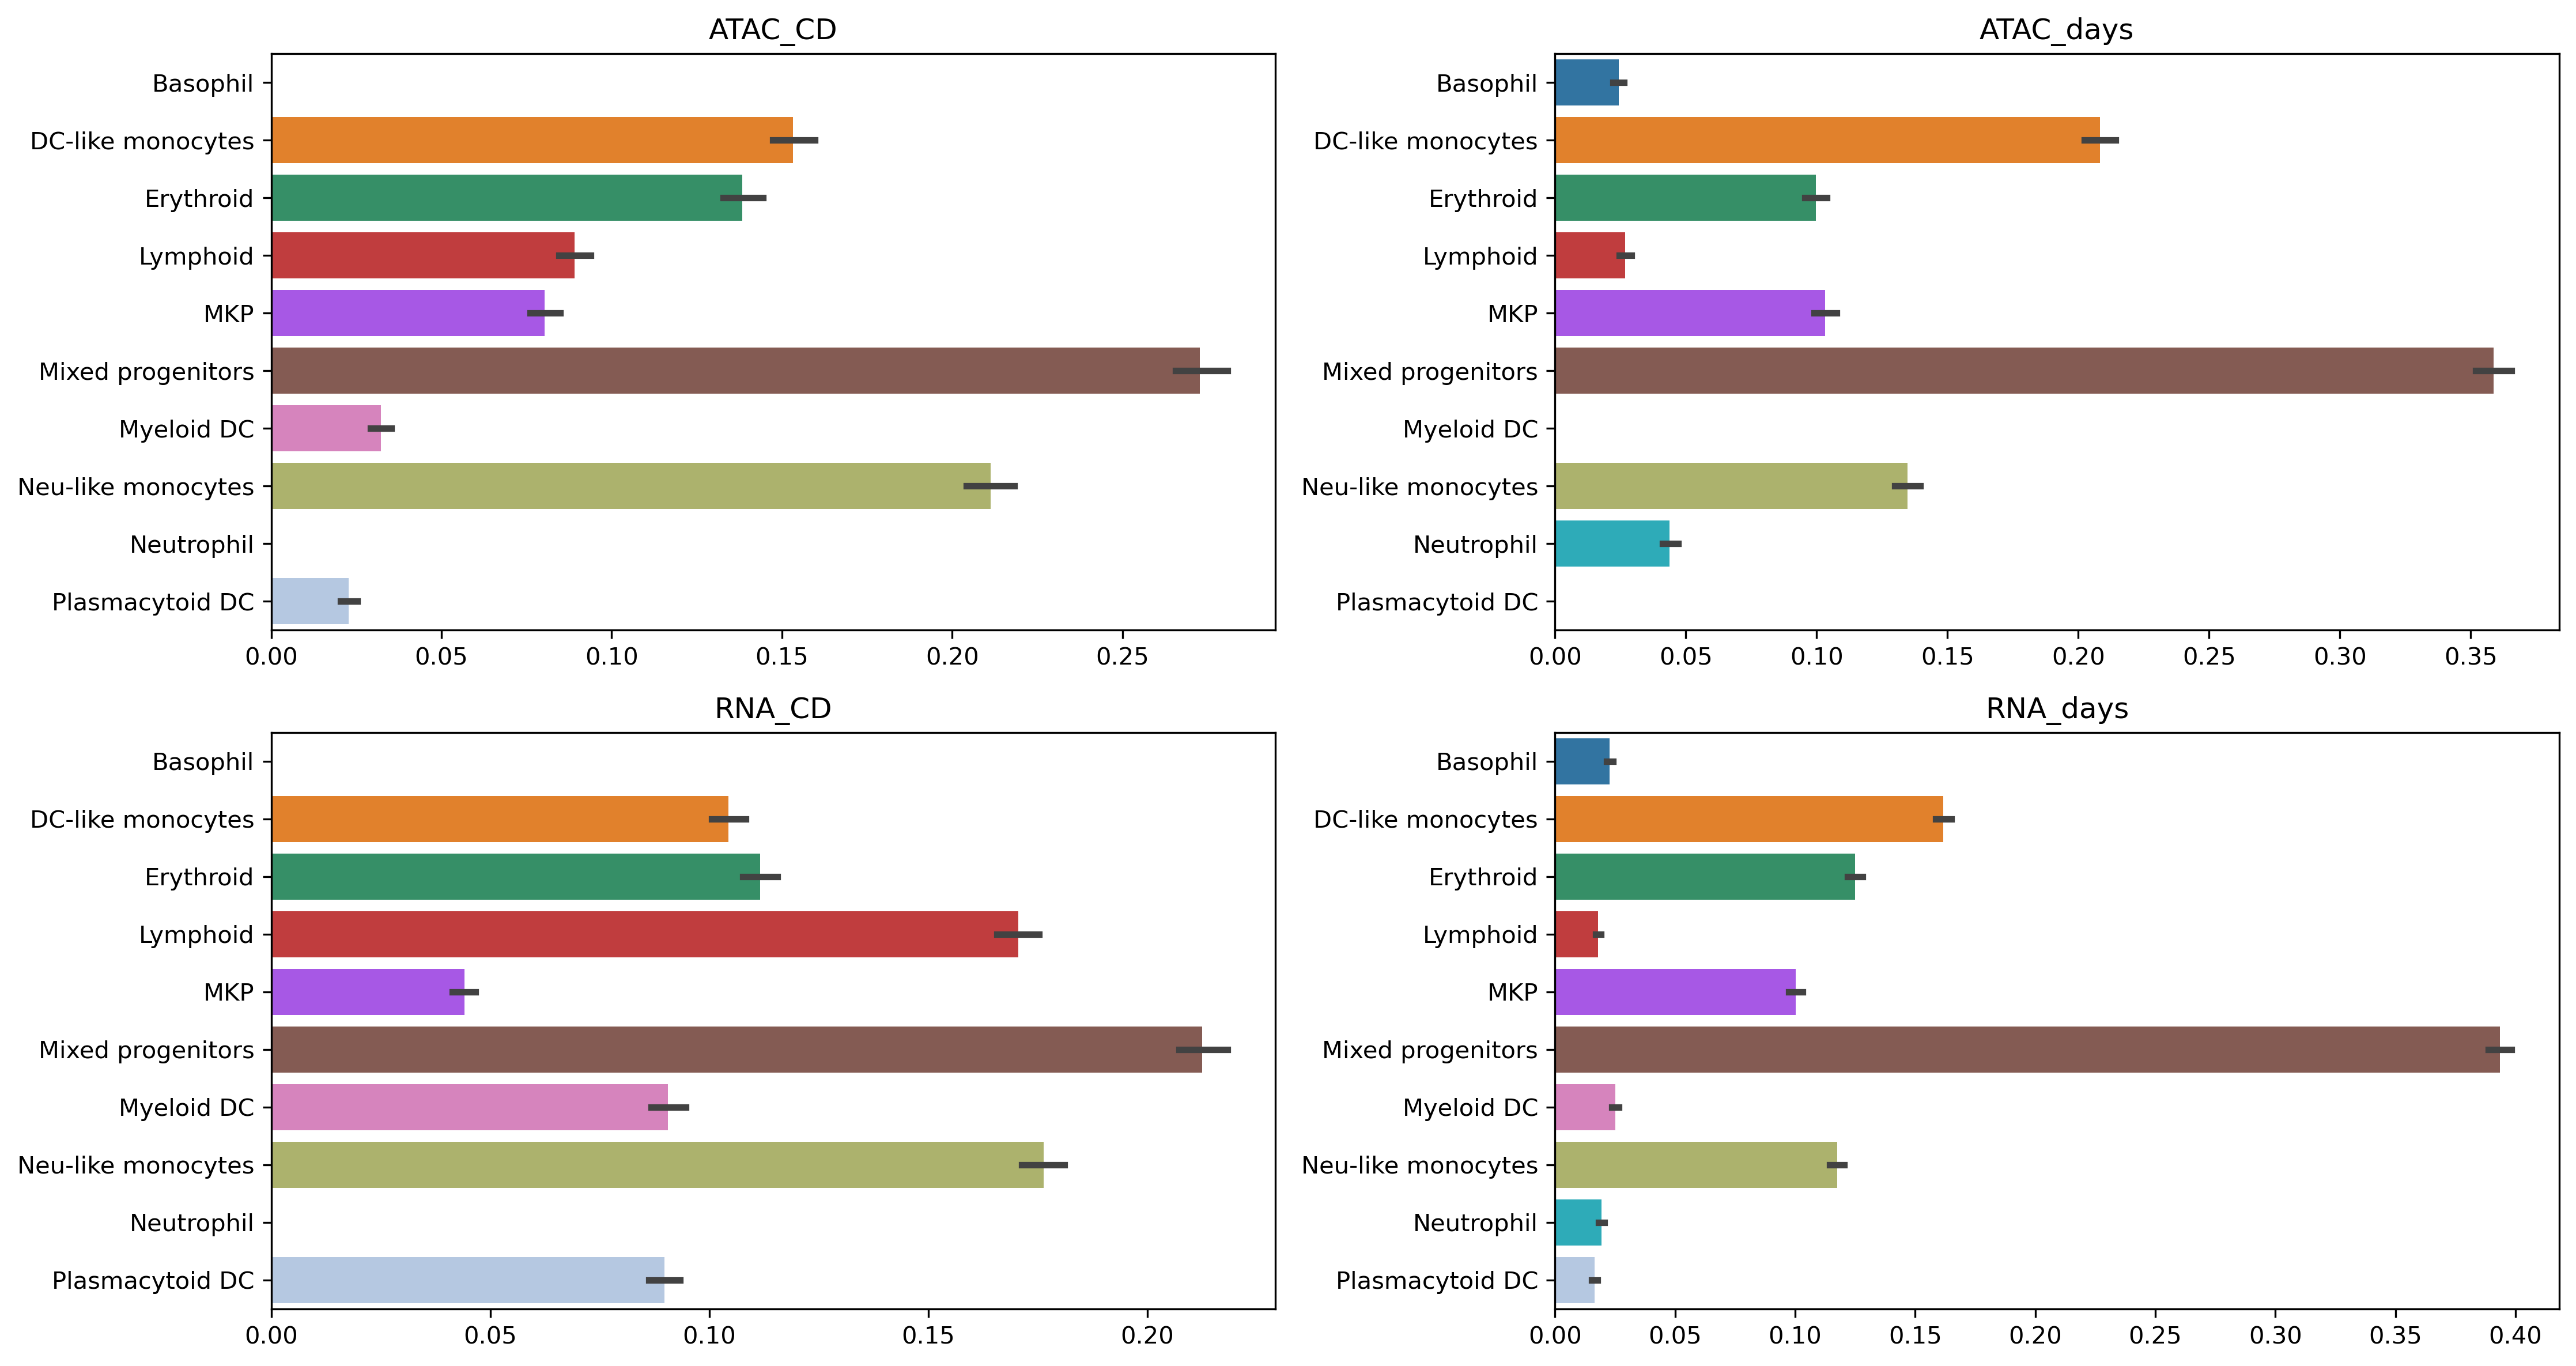
\includegraphics[width=\textwidth]{../figures/hematopoiesis/leiden_identity_simple2_proportions.png}
  \caption{Proportions: Leiden identity simple annotation}
\end{figure}

\begin{figure}[!htb]
  \centering
  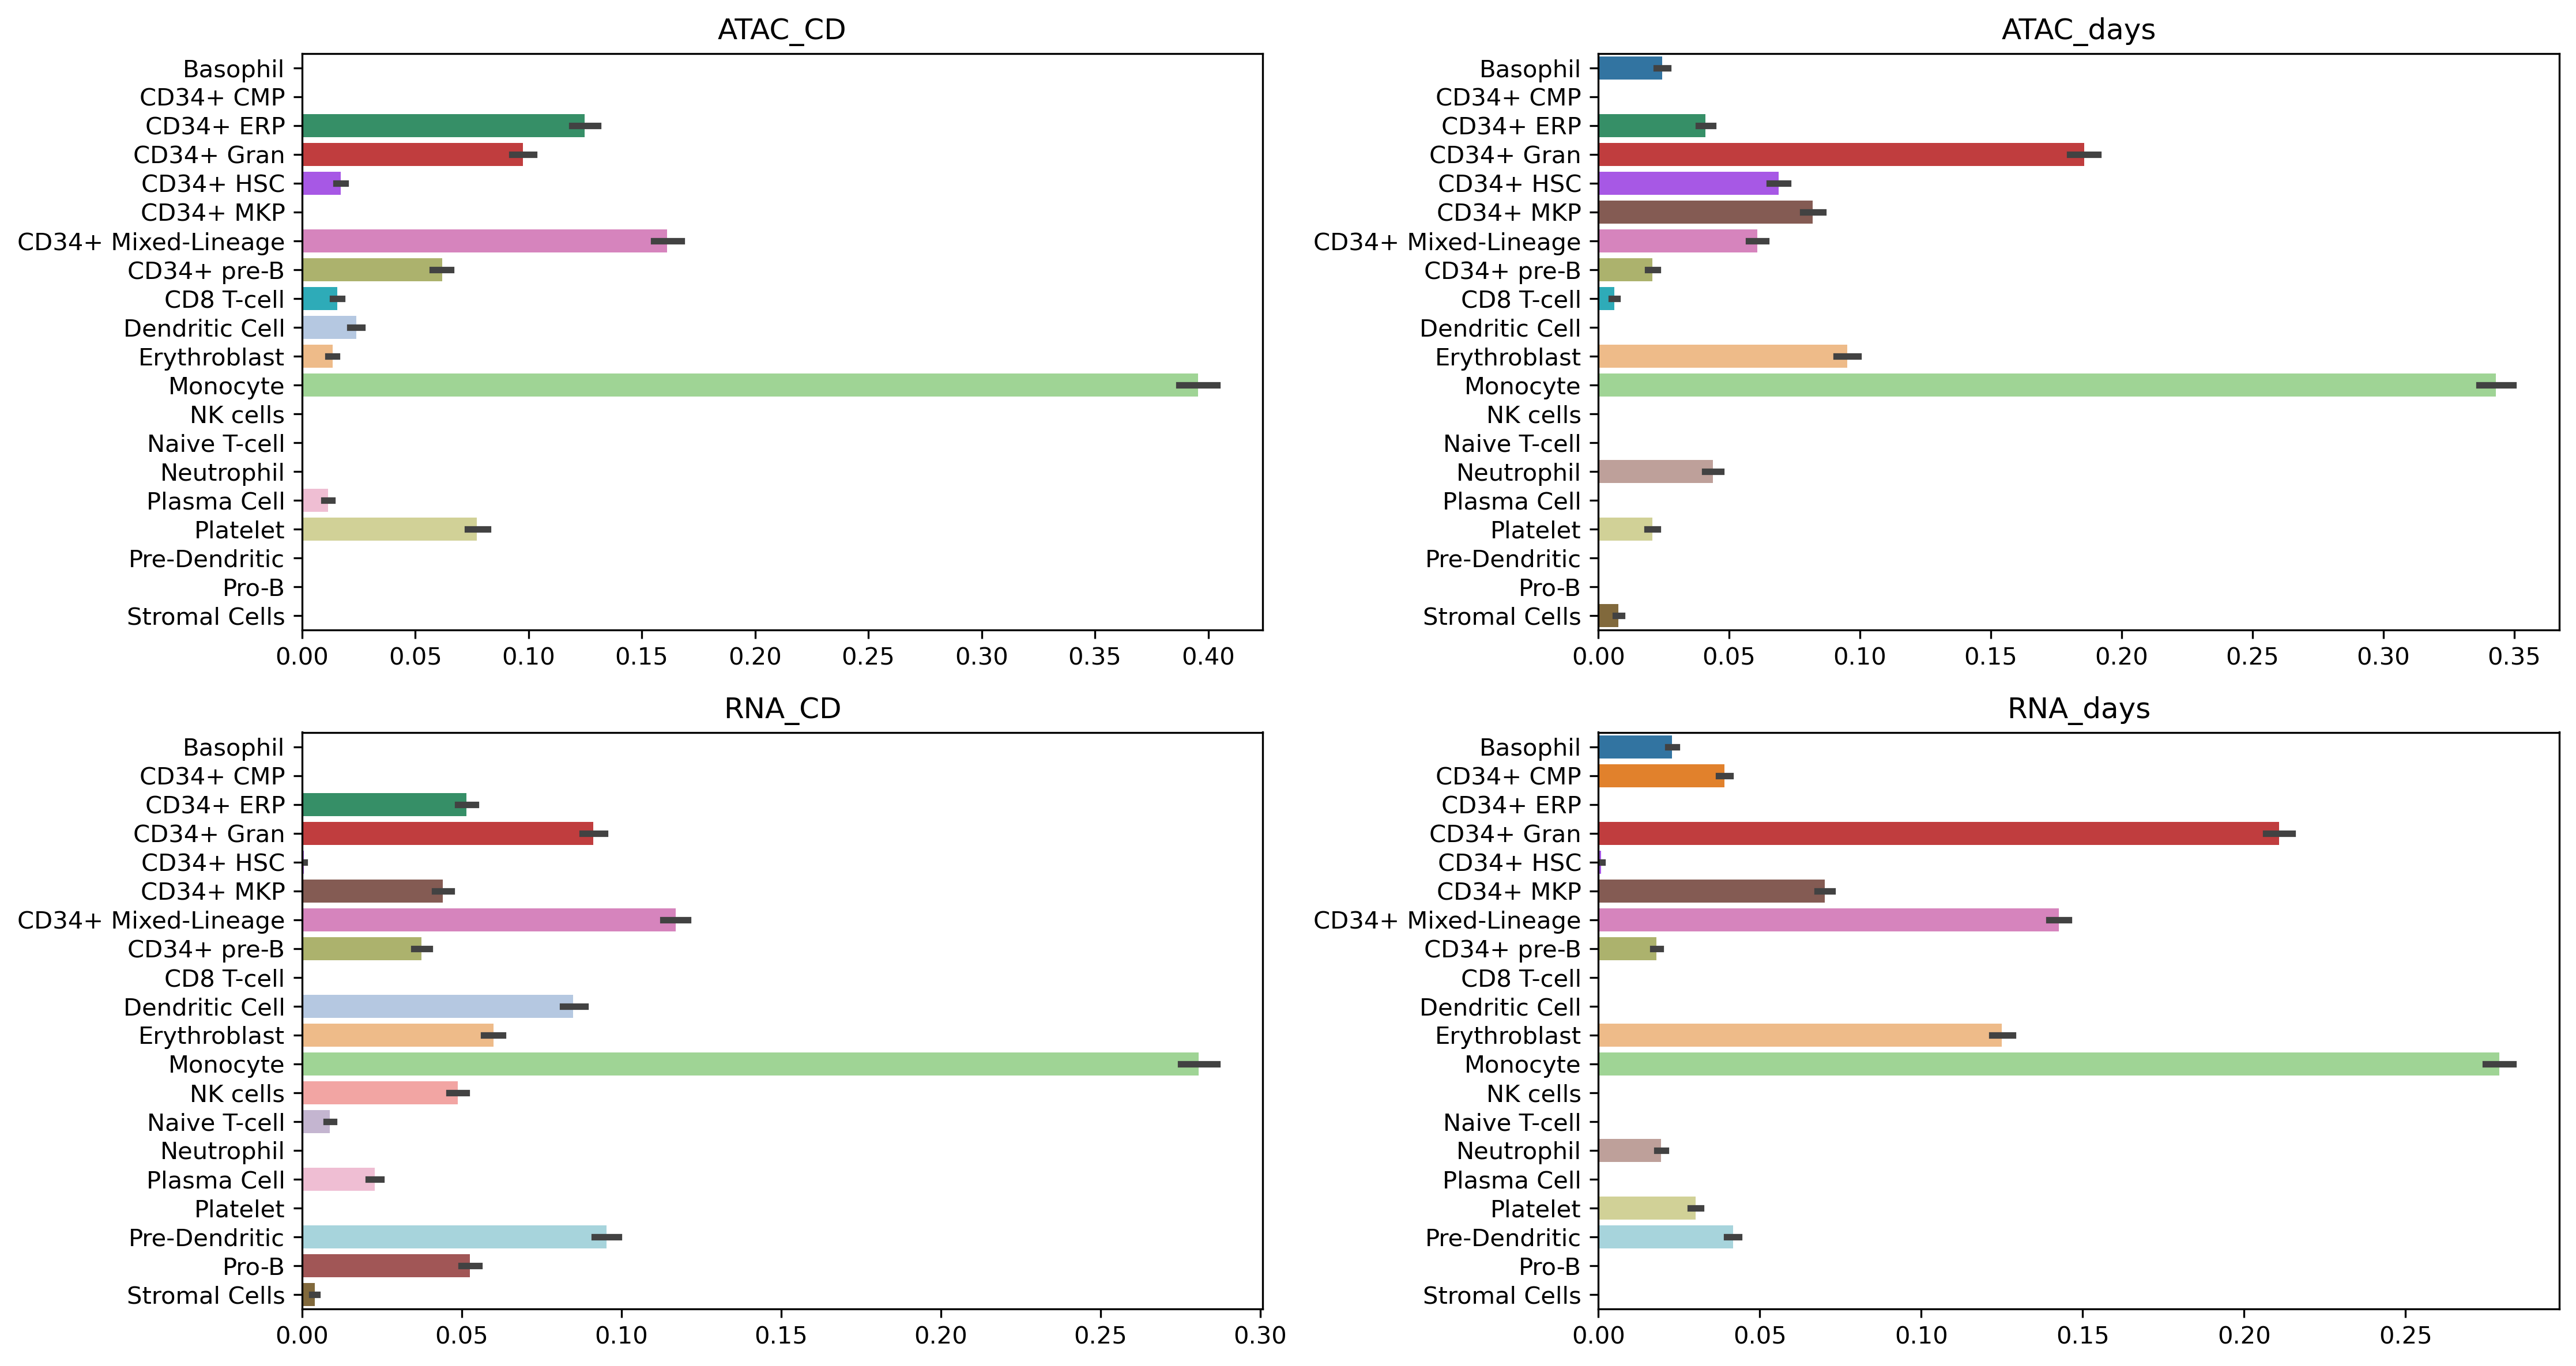
\includegraphics[width=\textwidth]{../figures/hematopoiesis/leiden_identity_proportions.png}
  \caption{Proportions: Leiden identity annotation}
\end{figure}

\FloatBarrier
\subsection{Correlation plots}

\begin{figure}[!htb]
  \centering
  \subfloat[RNA CD]{
    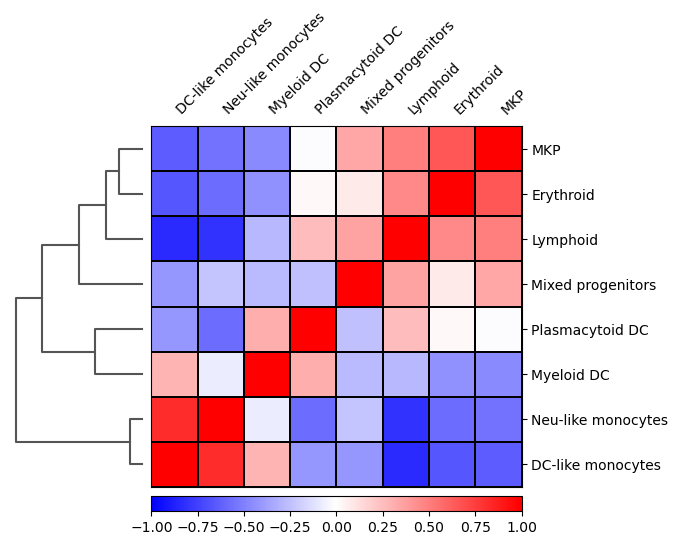
\includegraphics[width=0.5\textwidth]{../figures/hematopoiesis/correlation_matrix_leiden_identity_simple2_adata_RNA_CD.png}
  }
  \subfloat[RNA days]{
    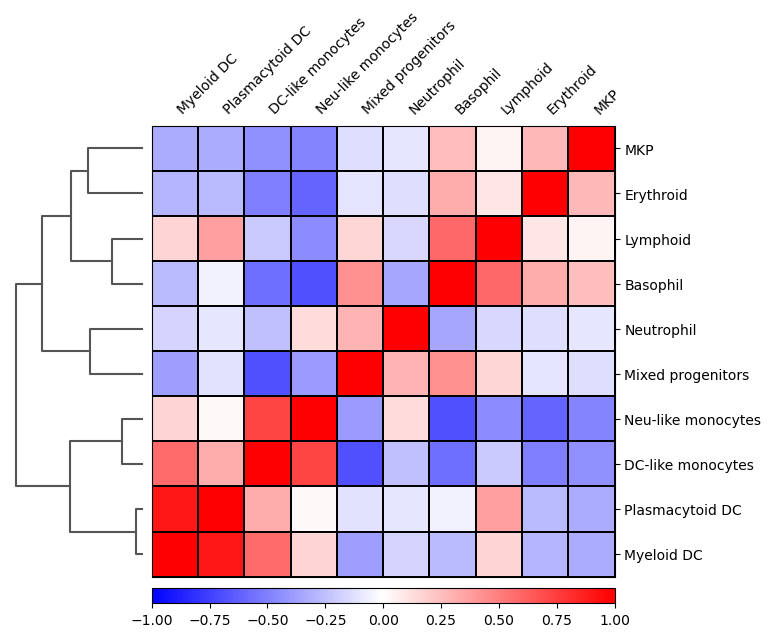
\includegraphics[width=0.5\textwidth]{../figures/hematopoiesis/correlation_matrix_leiden_identity_simple2_adata_RNA_days.png}
  }
  \hspace{0mm}
  \subfloat[ATAC CD]{
    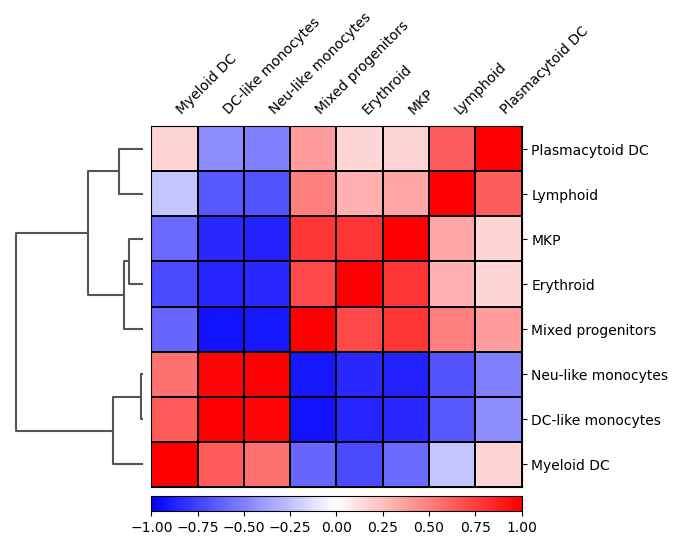
\includegraphics[width=0.5\textwidth]{../figures/hematopoiesis/correlation_matrix_leiden_identity_simple2_adata_ATAC_CD.png}
  }
  \subfloat[ATAC days]{
    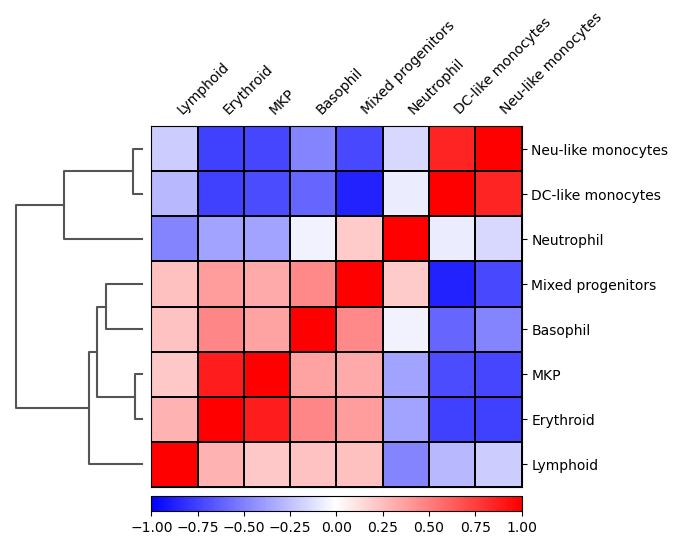
\includegraphics[width=0.5\textwidth]{../figures/hematopoiesis/correlation_matrix_leiden_identity_simple2_adata_ATAC_days.png}
  }
  \caption{Correlation between cell type averages (obtained using top PCs)}
\end{figure}

\FloatBarrier
\section{Data integration}

\subsection{Linear optimal transport}

\subsubsection{Scatter plots}
\begin{figure}[!htb]
  \centering
  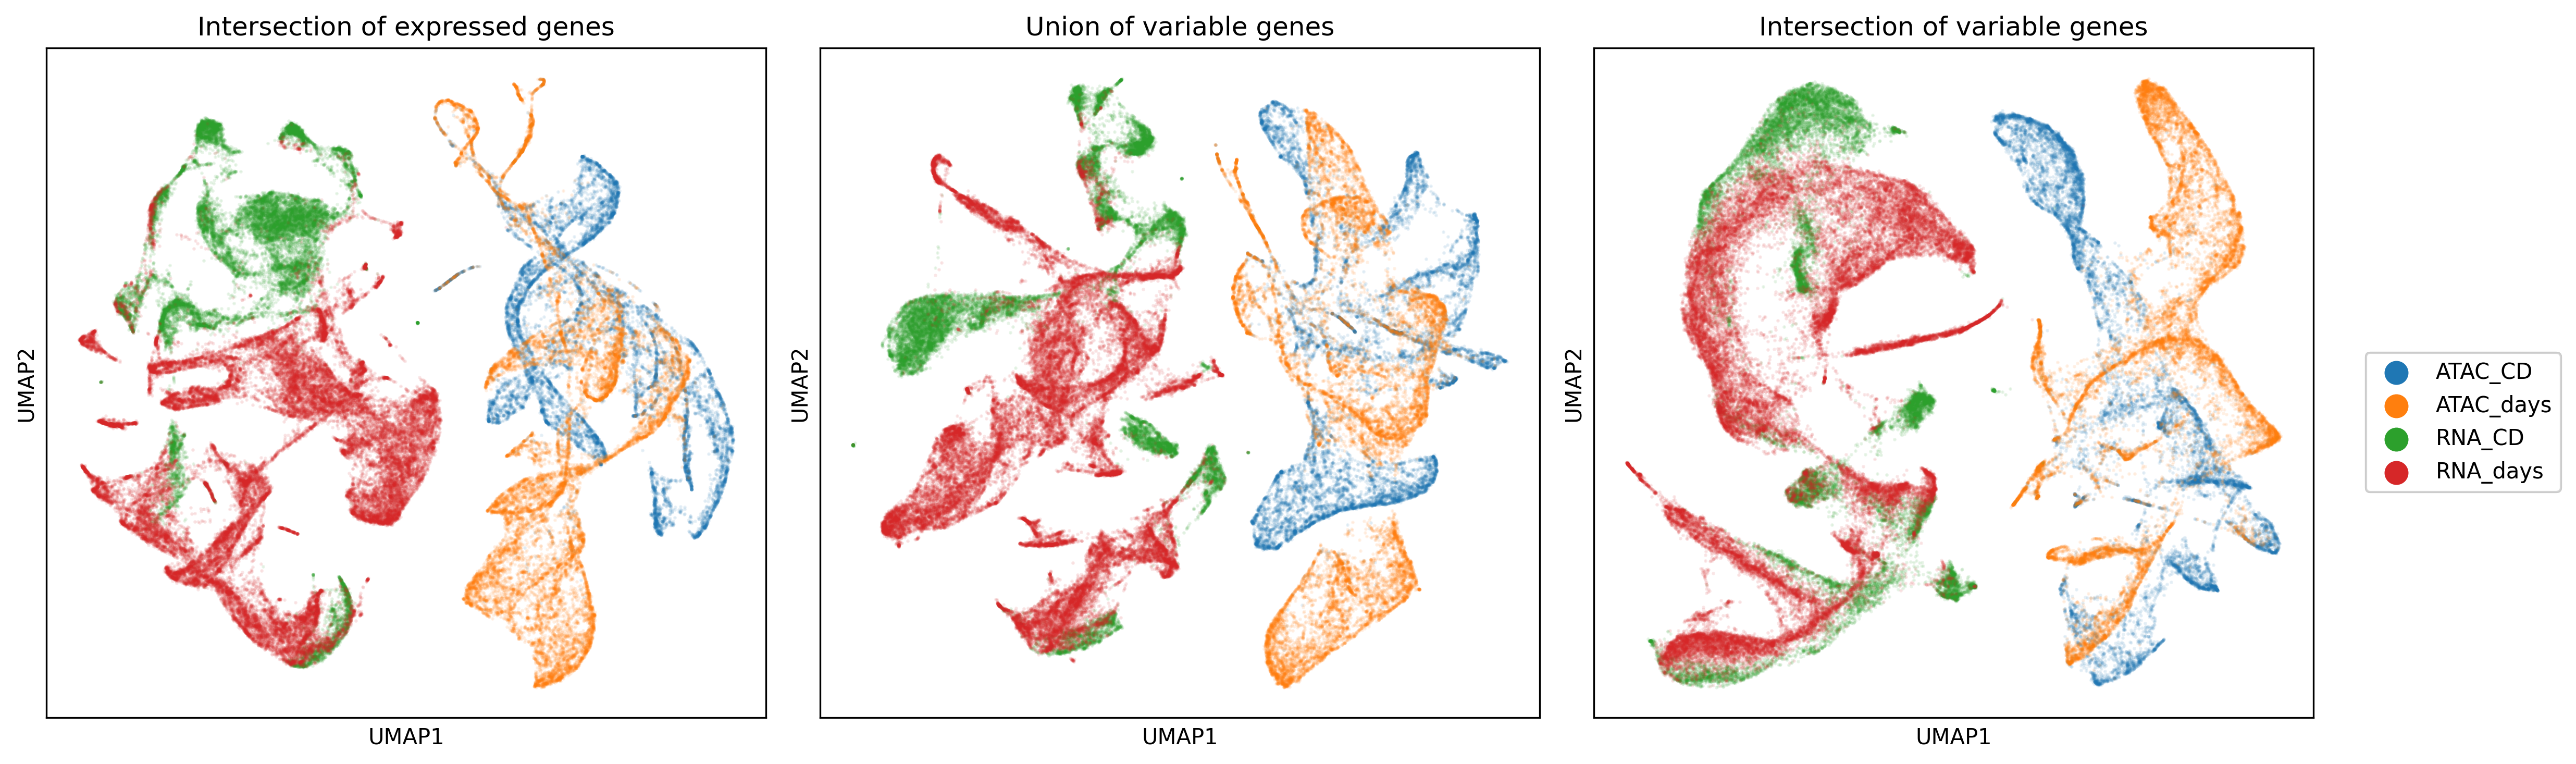
\includegraphics[width=\textwidth]{../figures/hematopoiesis/assays_RNA_days_subspace.png}
  \caption{Assays in RNA days PCA subspace}
\end{figure}

\begin{figure}[!htb]
  \centering
  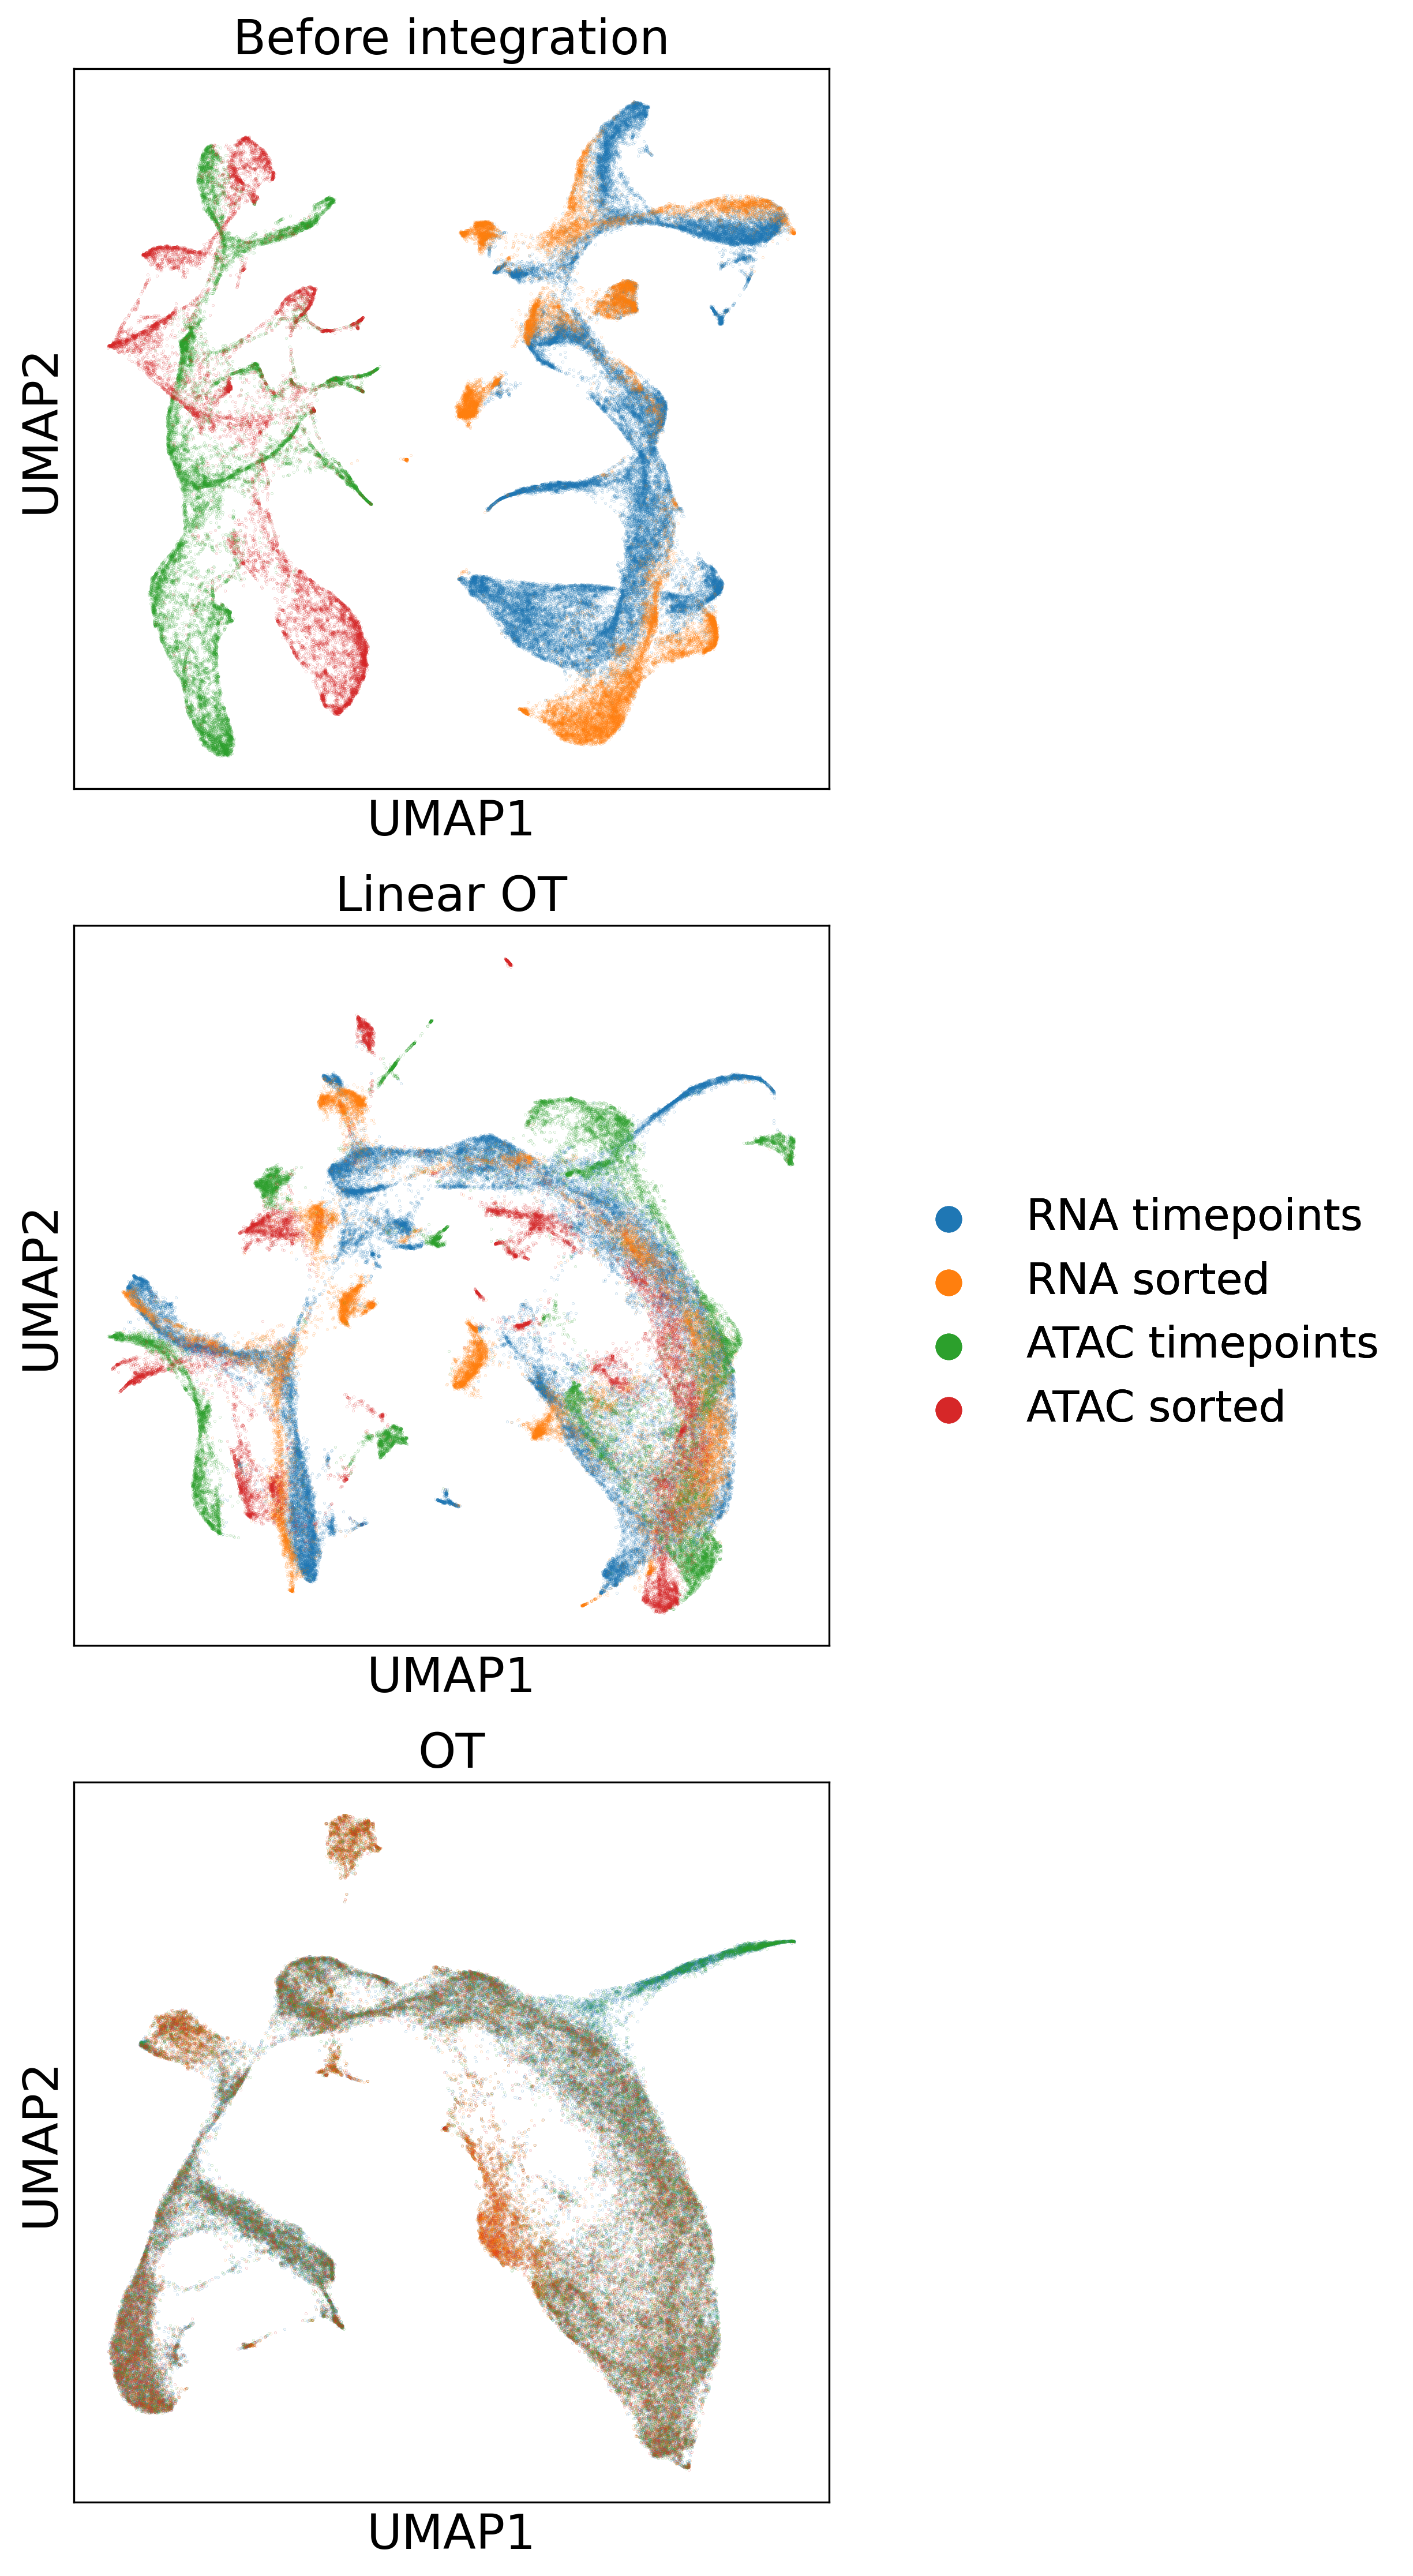
\includegraphics[width=\textwidth]{../figures/hematopoiesis/assays_RNA_days_subspace_aligned.png}
  \caption{Assays in RNA days PCA subspace, after alignment with linear optimal transport}
\end{figure}

\begin{figure}[!htb]
  \centering
  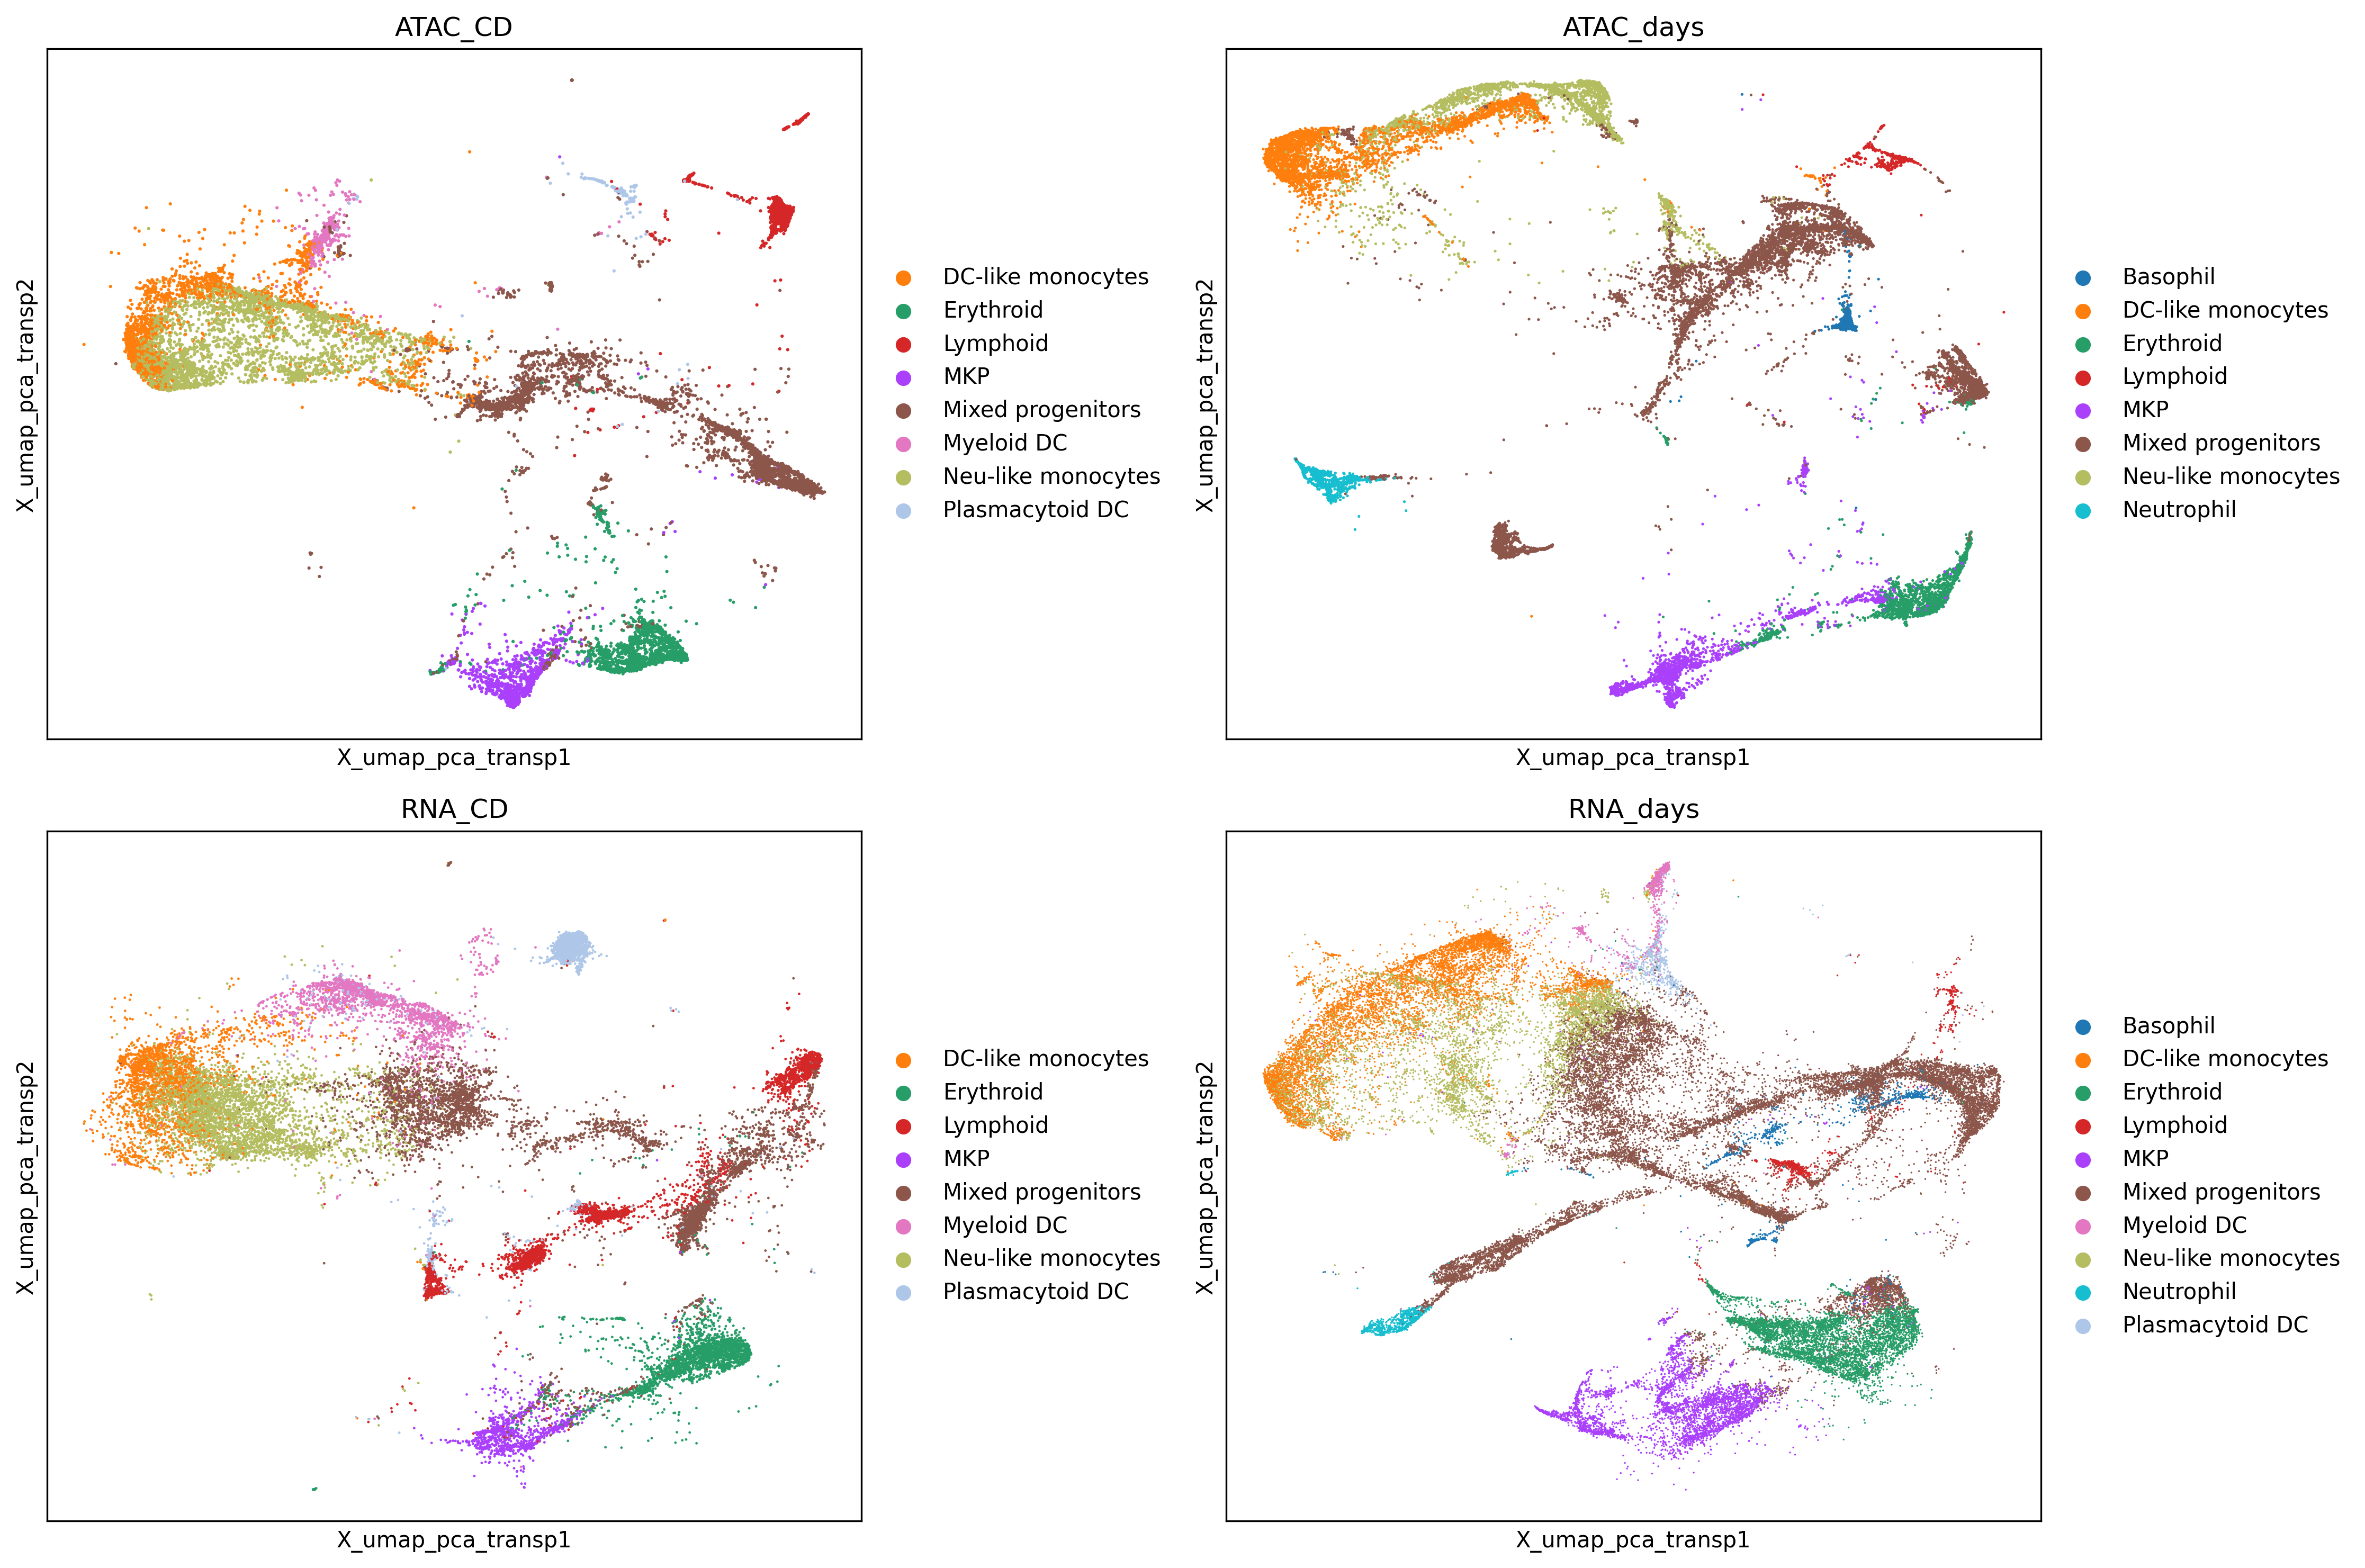
\includegraphics[width=\textwidth]{../figures/hematopoiesis/assays_RNA_days_subspace_aligned_Intersection_of_expressed_genes_leiden_identity_simple2.png}
  \caption{Assays in RNA days PCA subspace obtained using the intersection of expressed genes, after alignment with linear optimal transport.}
\end{figure}

\begin{figure}[!htb]
  \centering
  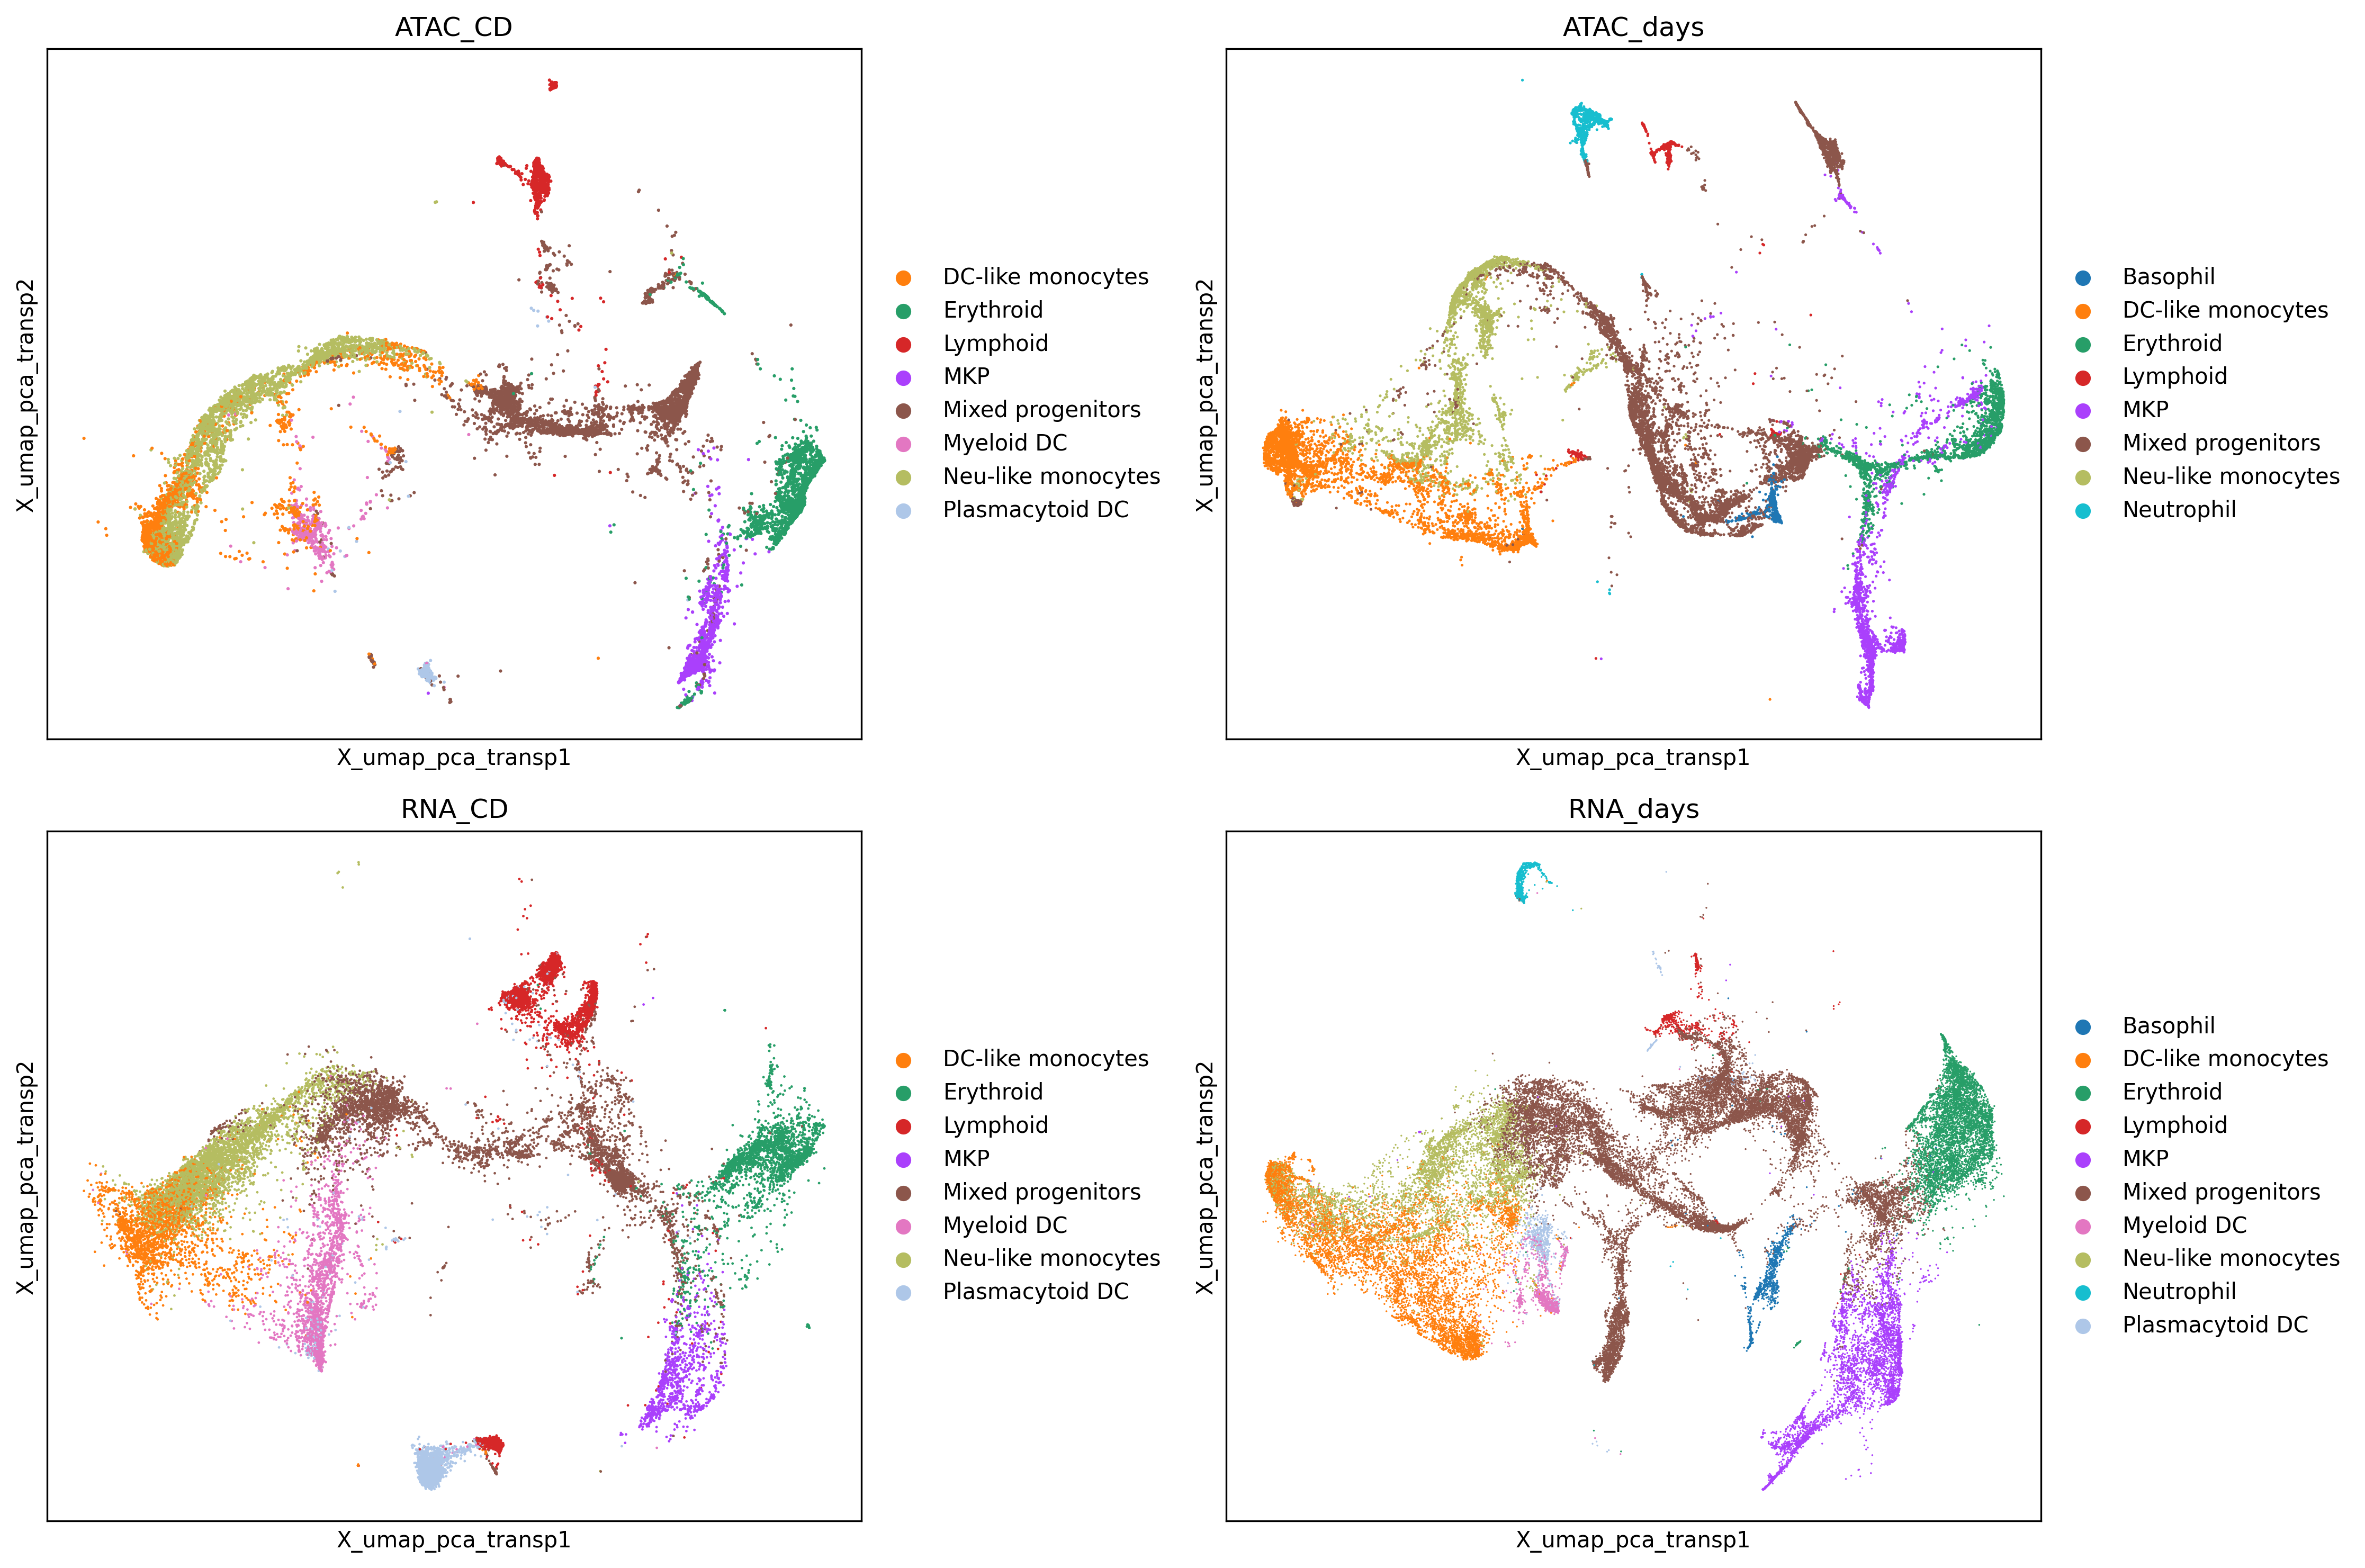
\includegraphics[width=\textwidth]{../figures/hematopoiesis/assays_RNA_days_subspace_aligned_Union_of_variable_genes_leiden_identity_simple2.png}
  \caption{Assays in RNA days PCA subspace obtained using the union of variable genes, after alignment with linear optimal transport.}
\end{figure}

\begin{figure}[!htb]
  \centering
  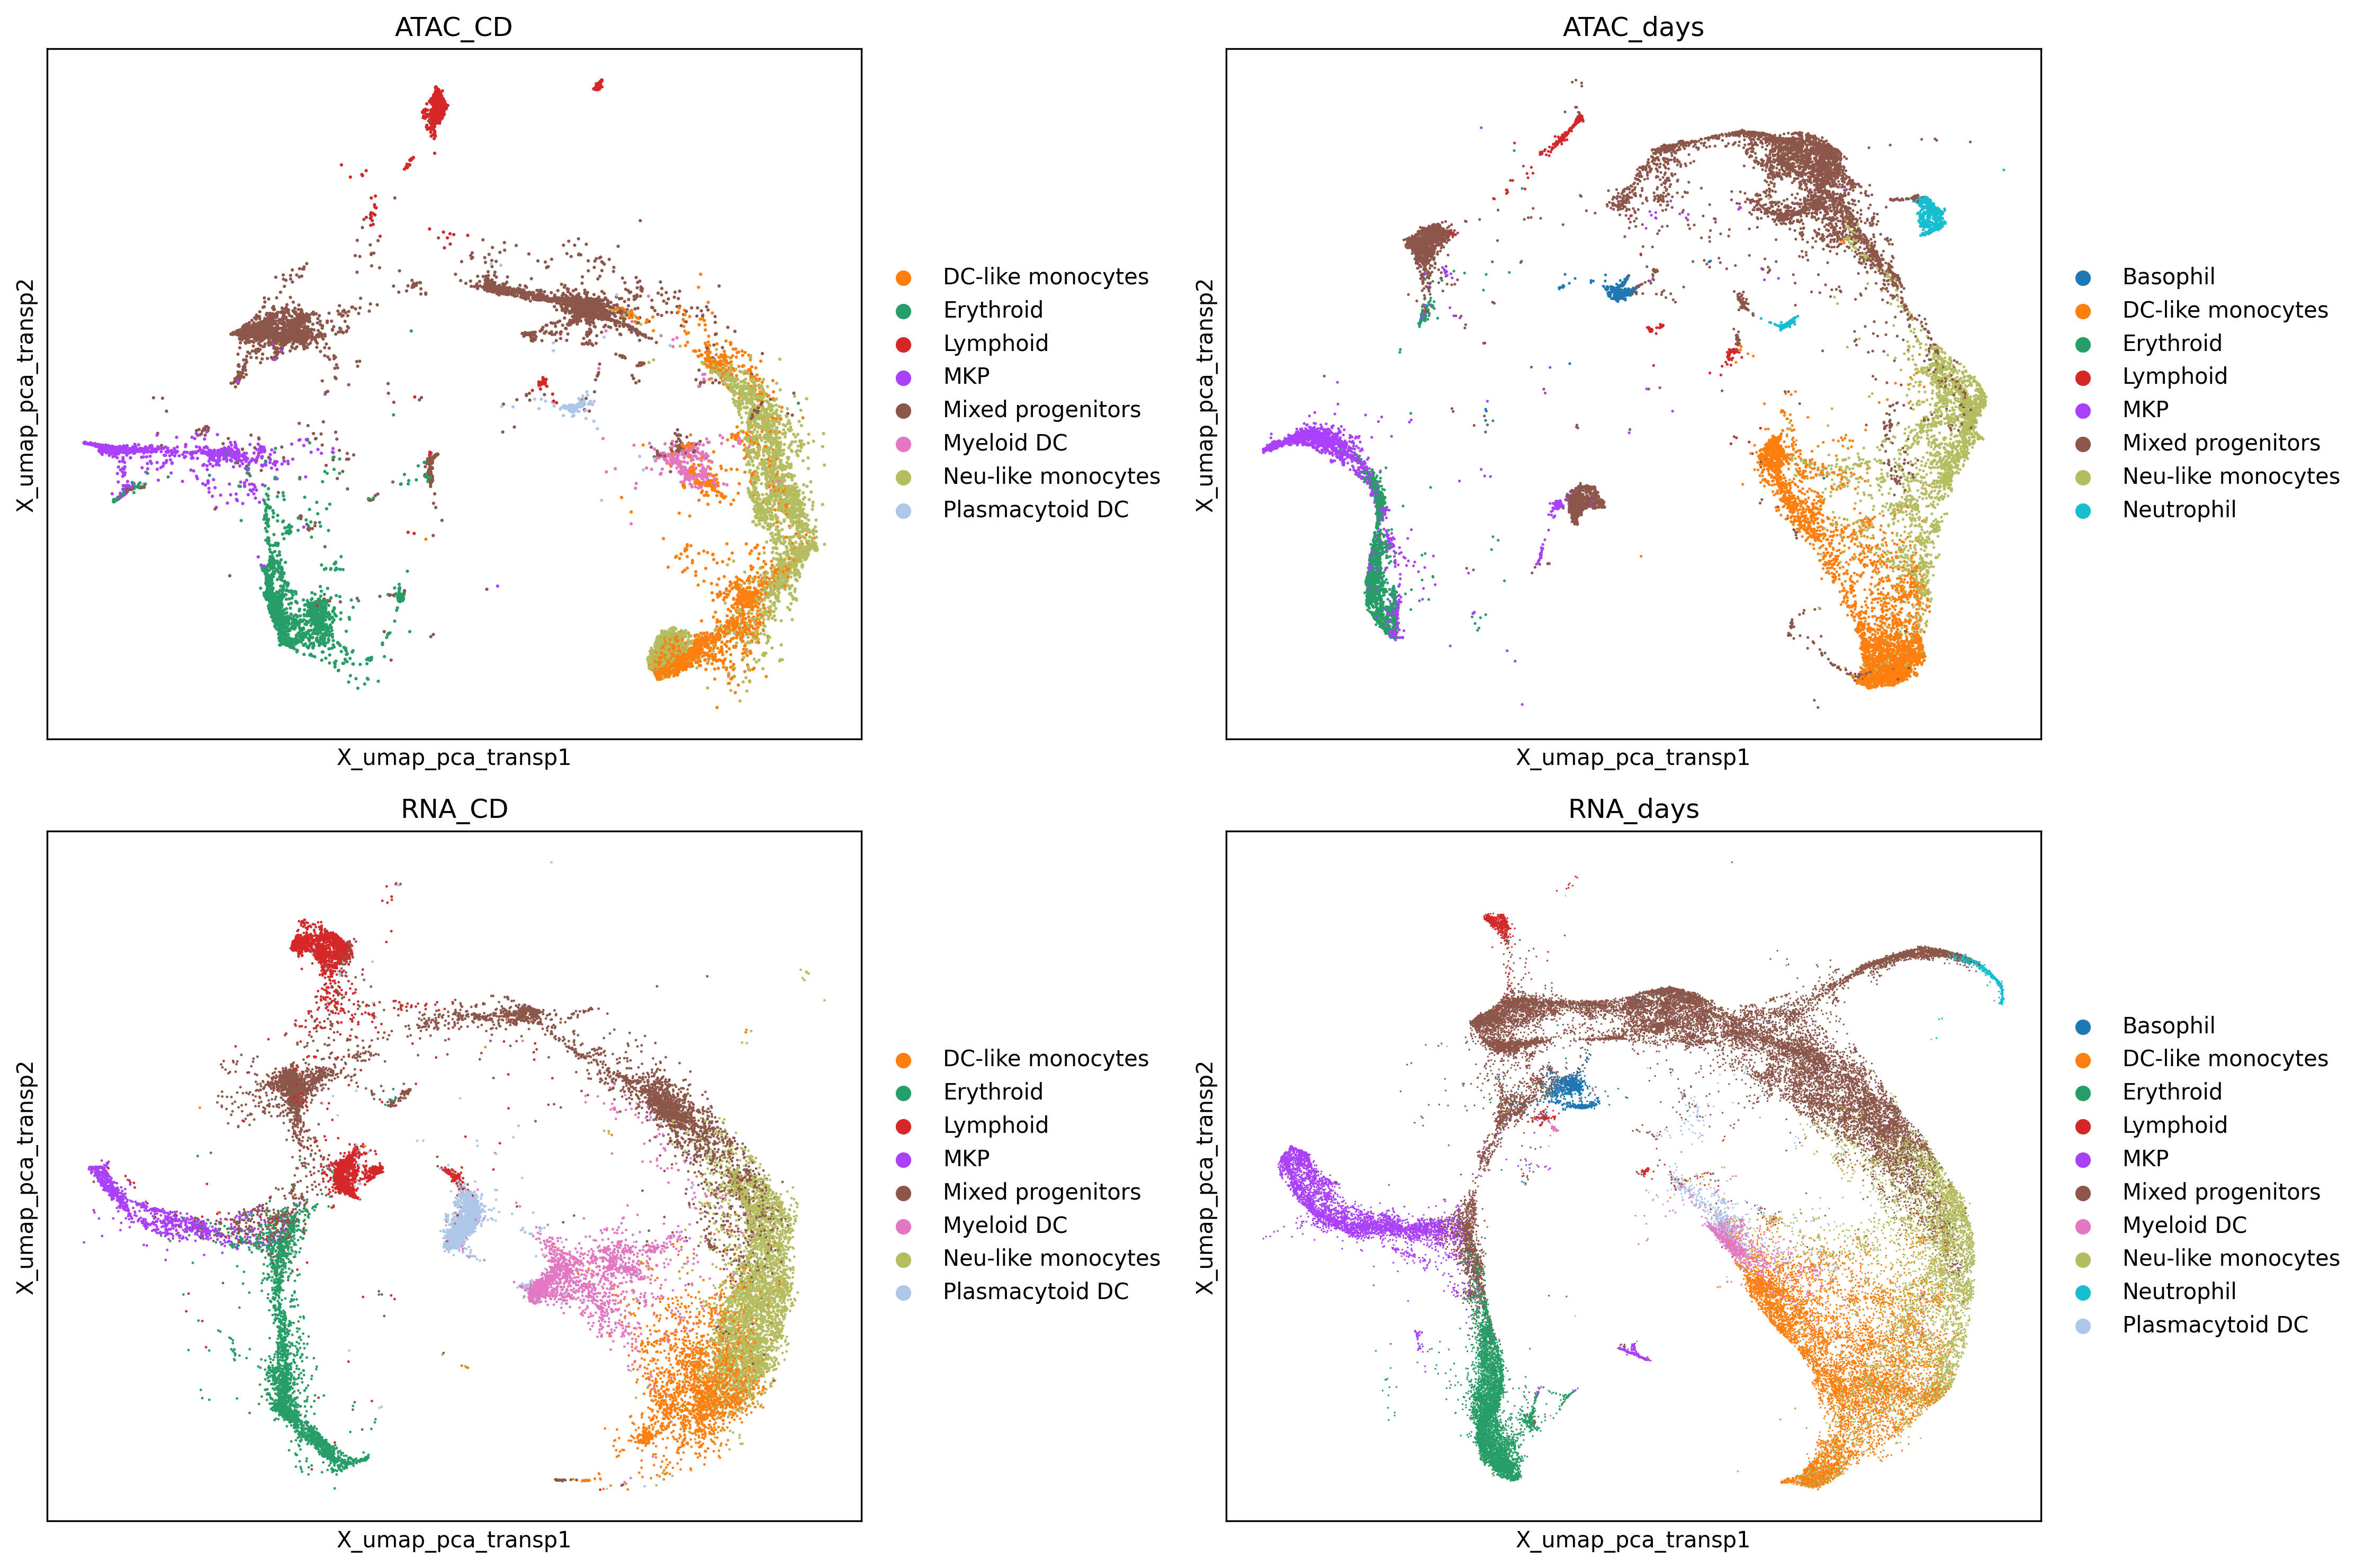
\includegraphics[width=\textwidth]{../figures/hematopoiesis/assays_RNA_days_subspace_aligned_Intersection_of_variable_genes_leiden_identity_simple2.png}
  \caption{Assays in RNA days PCA subspace obtained using the intersection of variable genes, after alignment with linear optimal transport.}
\end{figure}

\FloatBarrier
\subsubsection{Correlation plots}

\begin{figure}[!htb]
  \centering
  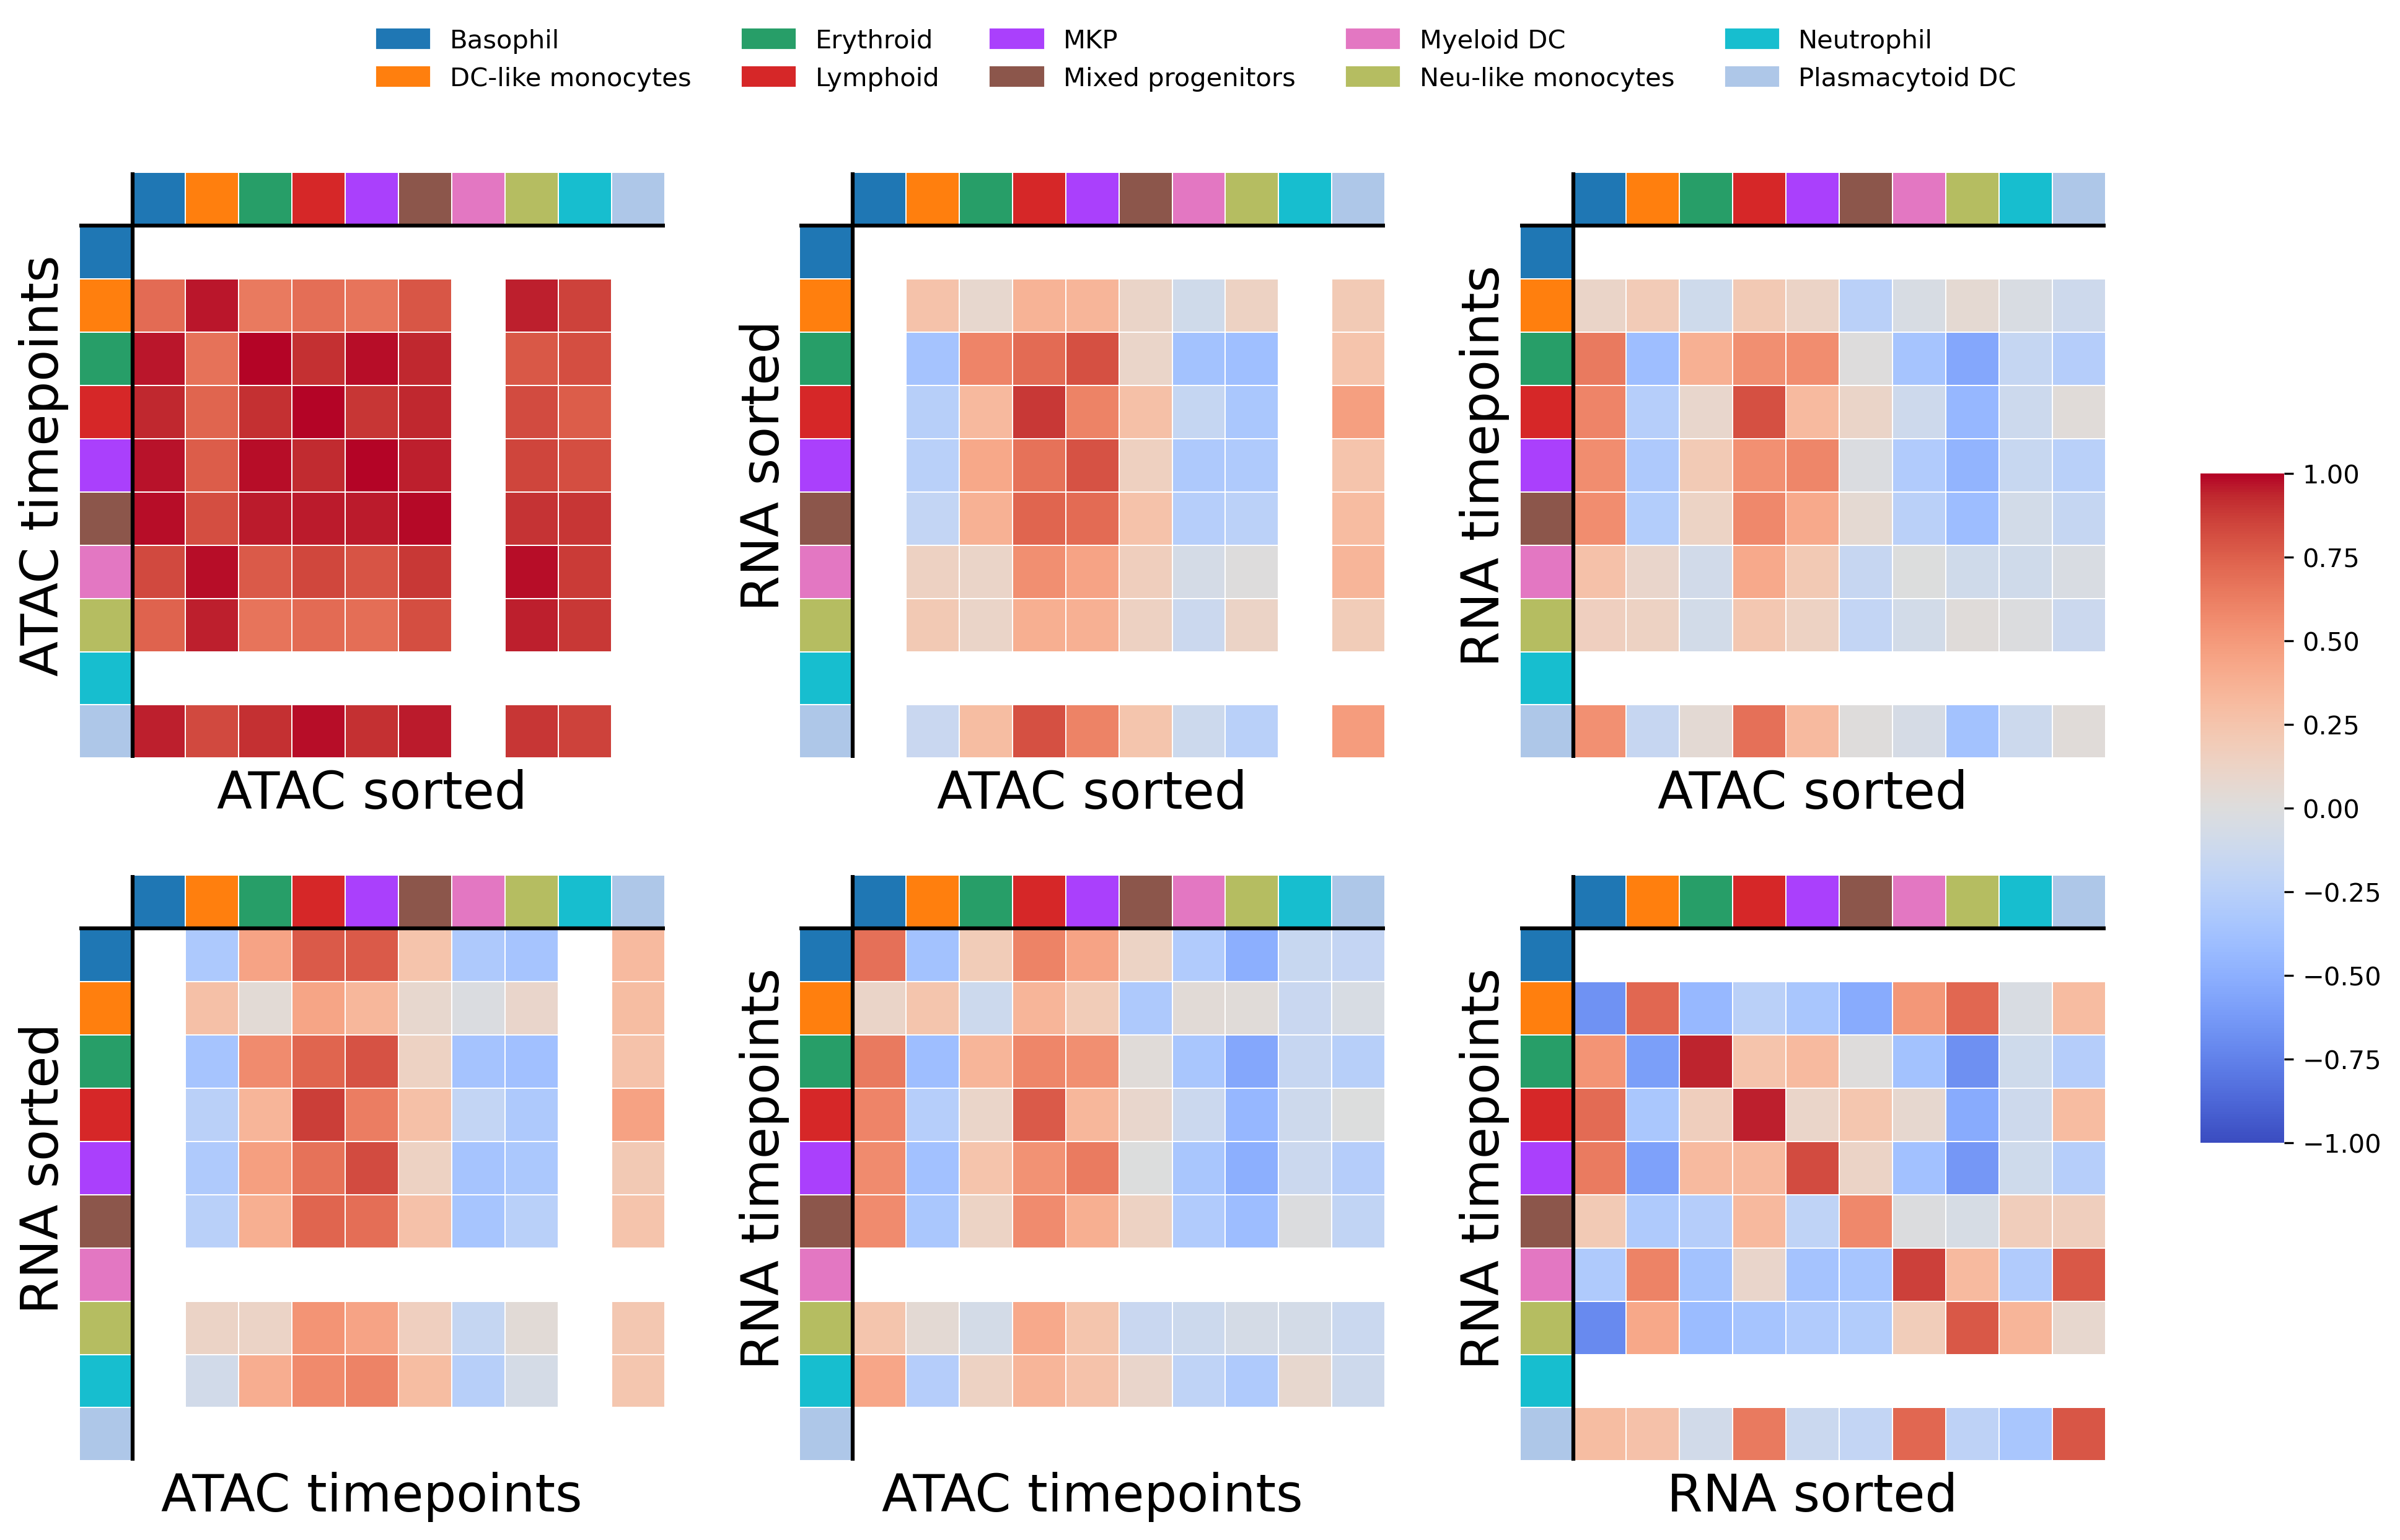
\includegraphics[width=\textwidth]{../figures/hematopoiesis/assays_X_pca_target_leiden_identity_simple2.png}
  \caption{Correlation between assays' cell type averages (obtained using top PCs of assays, each in their own PCA subspace)}
\end{figure}

\begin{figure}[!htb]
  \centering
  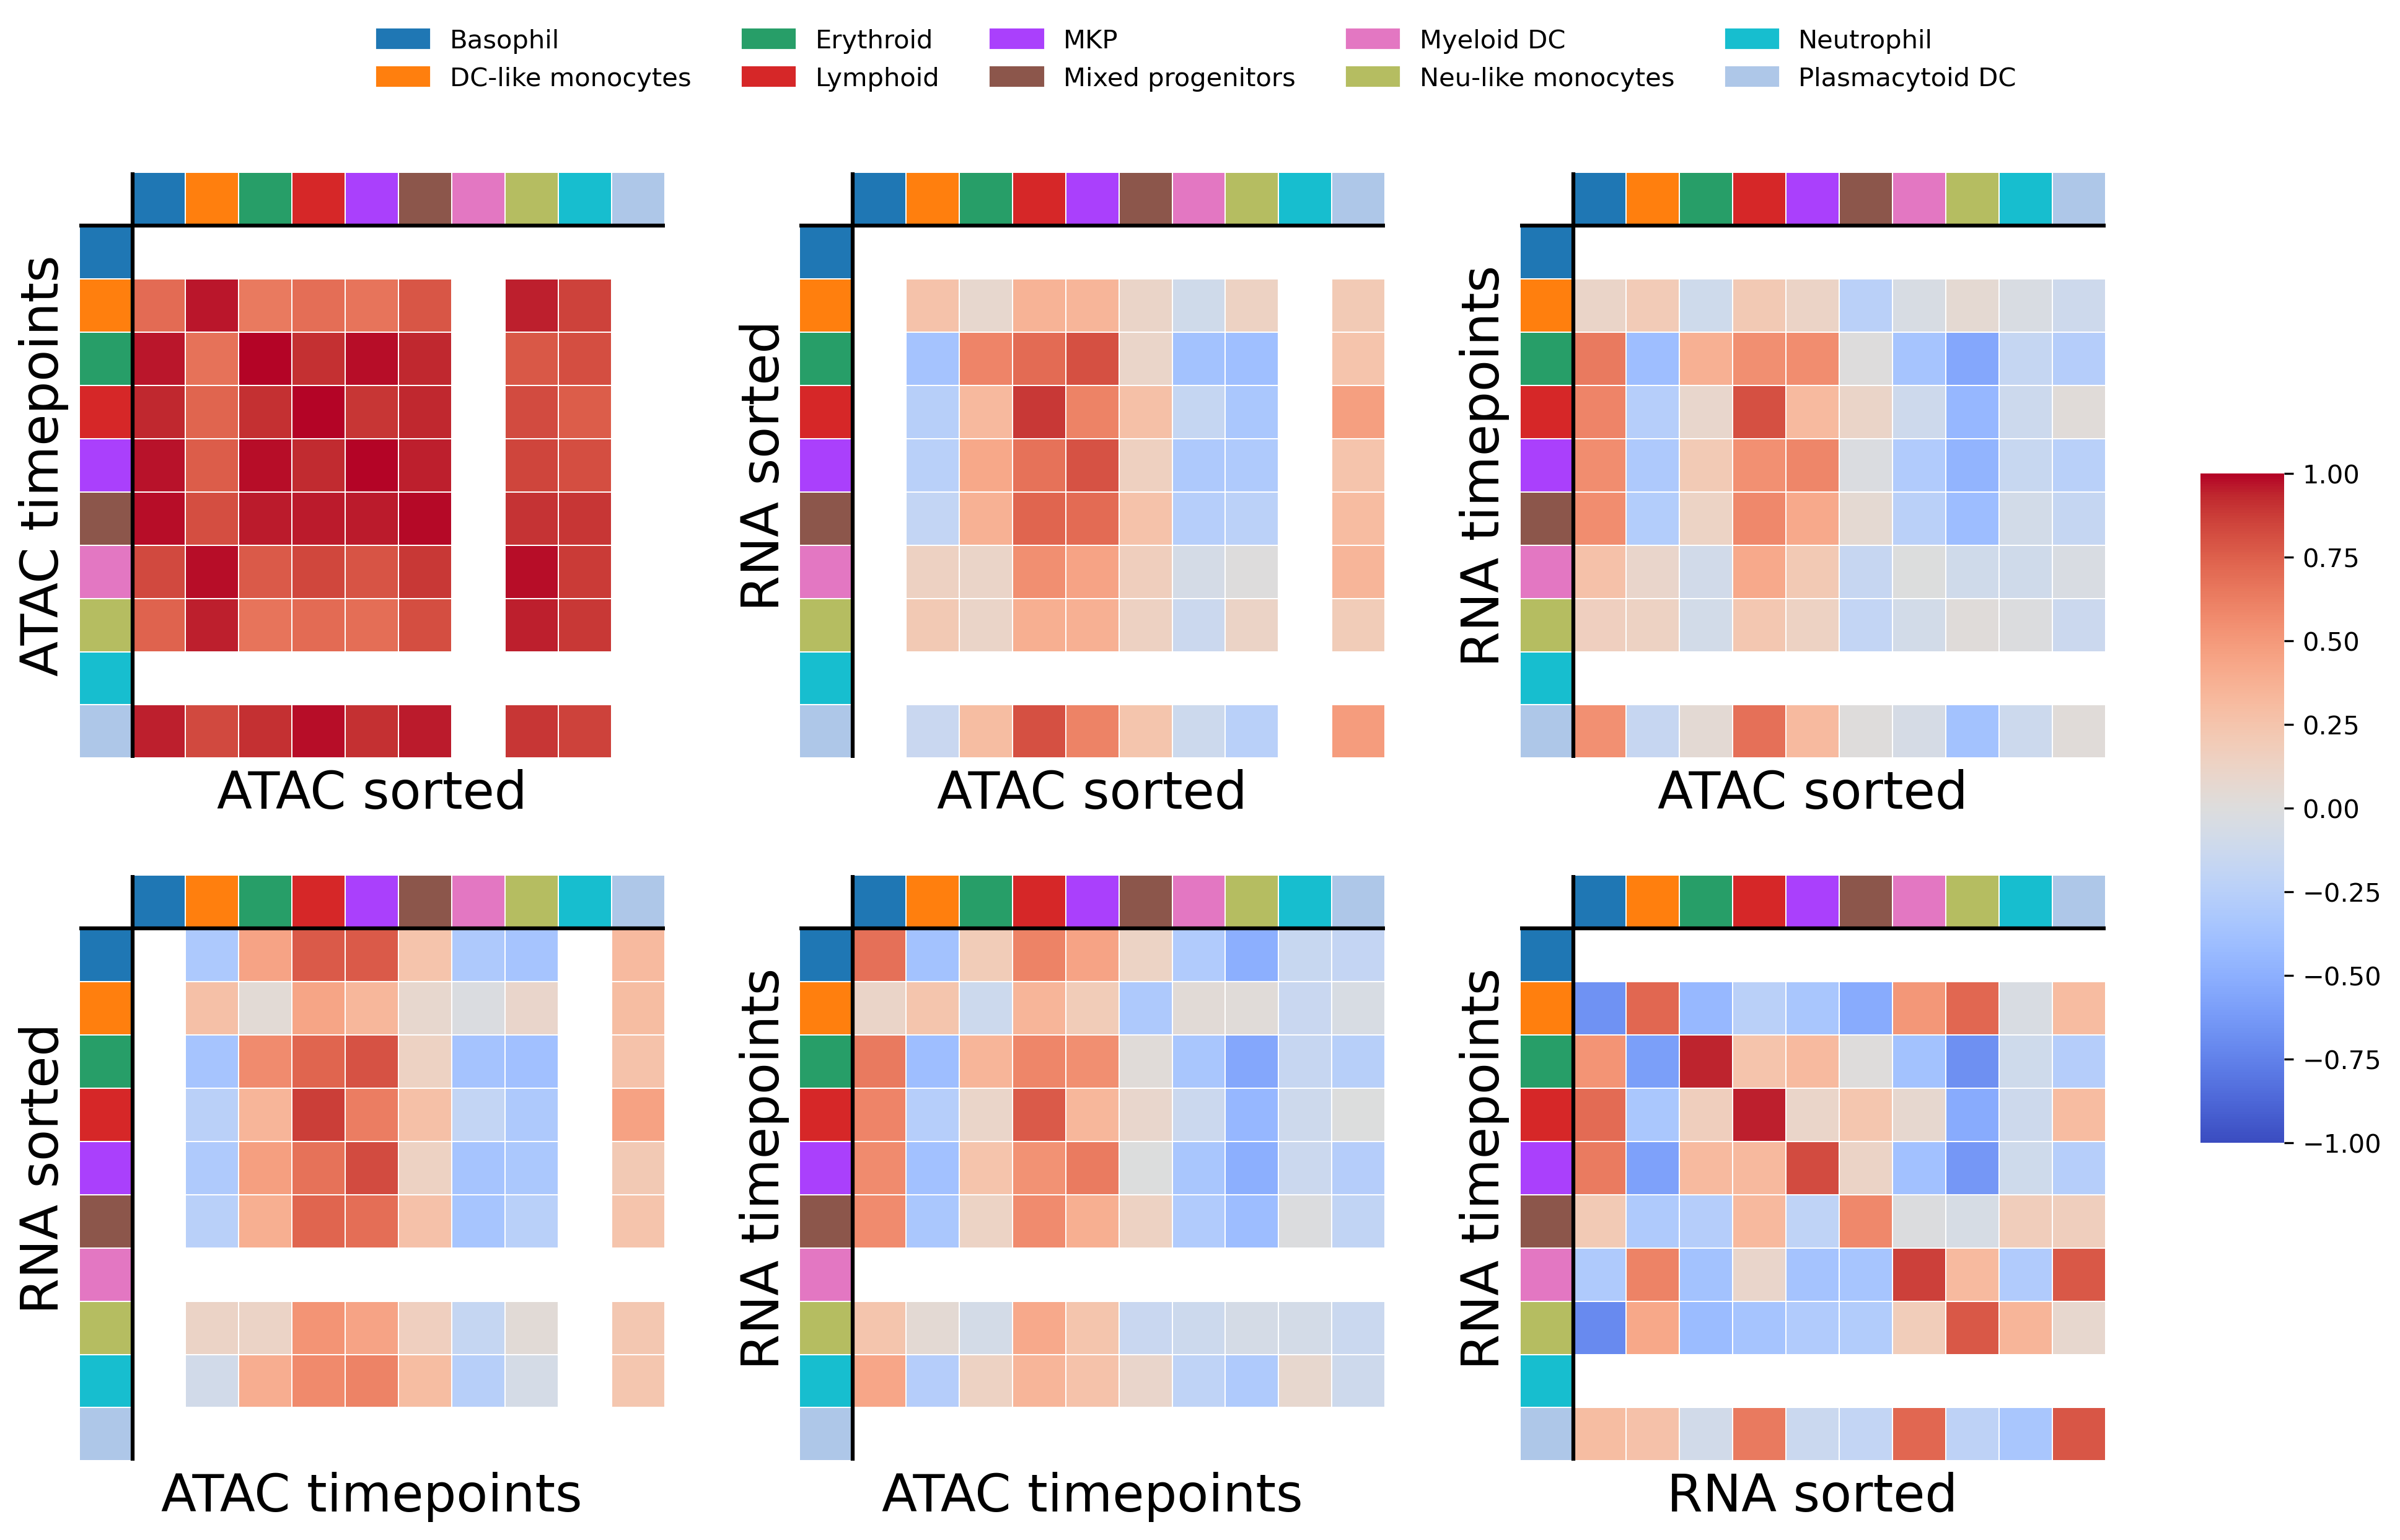
\includegraphics[width=\textwidth]{../figures/hematopoiesis/assays_X_pca_target_leiden_identity_simple2.png}
  \caption{Correlation between assays' cell type averages (obtained using top PCs of assays in RNA days PCA subspace)}
\end{figure}

\begin{figure}[!htb]
  \centering
  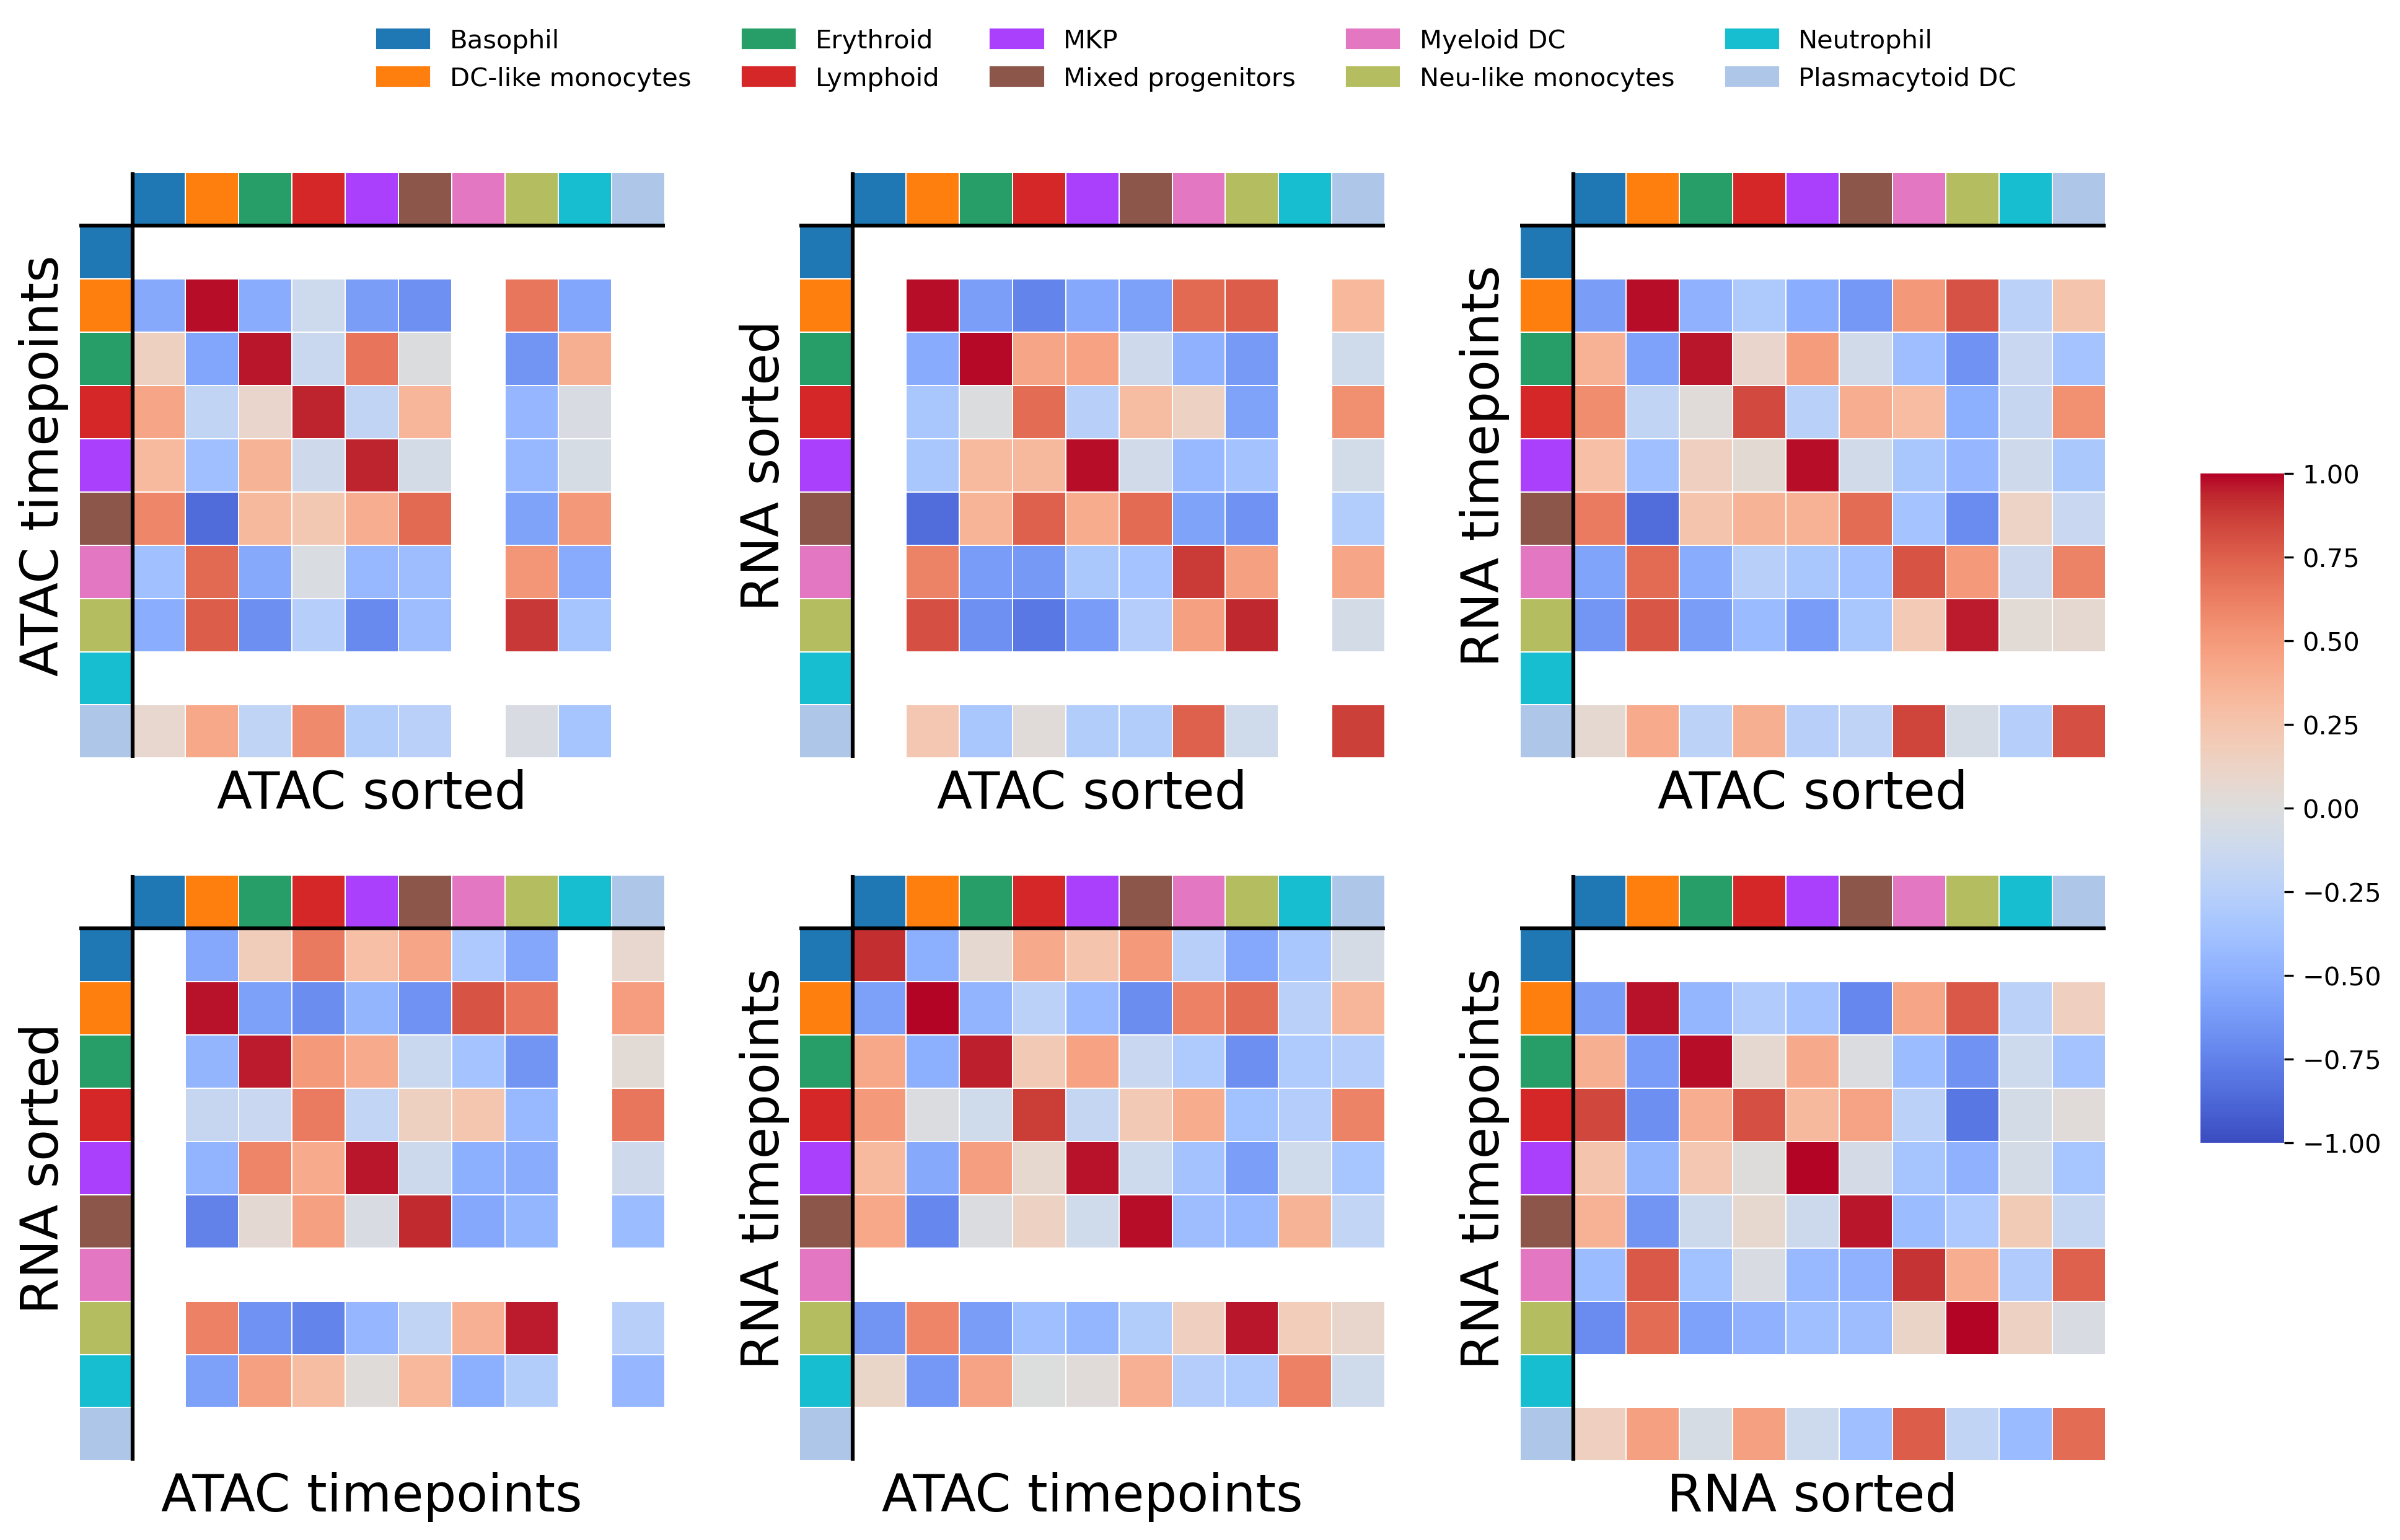
\includegraphics[width=\textwidth]{../figures/hematopoiesis/assays_X_pca_transp_leiden_identity_simple2.png}
  \caption{Correlation between assays' cell type averages (obtained using top PCs of assays in RNA days PCA subspace, after alignment with linear optimal transport)}
\end{figure}

\FloatBarrier
\subsection{Supervised optimal transport}

\textbf{Grouping of categories to go from full to simple annotation}
\begin{itemize}
  \item 'Early-ERP','Erythroblast','CD34+ ERP' = 'Erythroid'
  \item 'Platelet','CD34+ MKP' = 'MKP'
  \item 'Pre-Dendritic','Dendritic Cell' = 'Dendritic'
  \item 'CD34+ CLP','CD34+ pre-B','Pro-B','Plasma Cell', 'NK cells','Naive T-cell','CD8 T-cell' = 'Lymphoid'
  \item 'CD34+ Mixed-Lineage', 'CD34+ HSC','CD34+ CMP', 'CD34+ Gran', 'Eosinophil','Stromal Cells' = 'Mixed-Lineage'
  \item change unlikely 'Erythroid' annotation (outlier, mixed cluster) for late ATAC days (day 7 and 12) to 'Mixed-Lineage'
\end{itemize}

\begin{figure}[!htb]
  \centering
  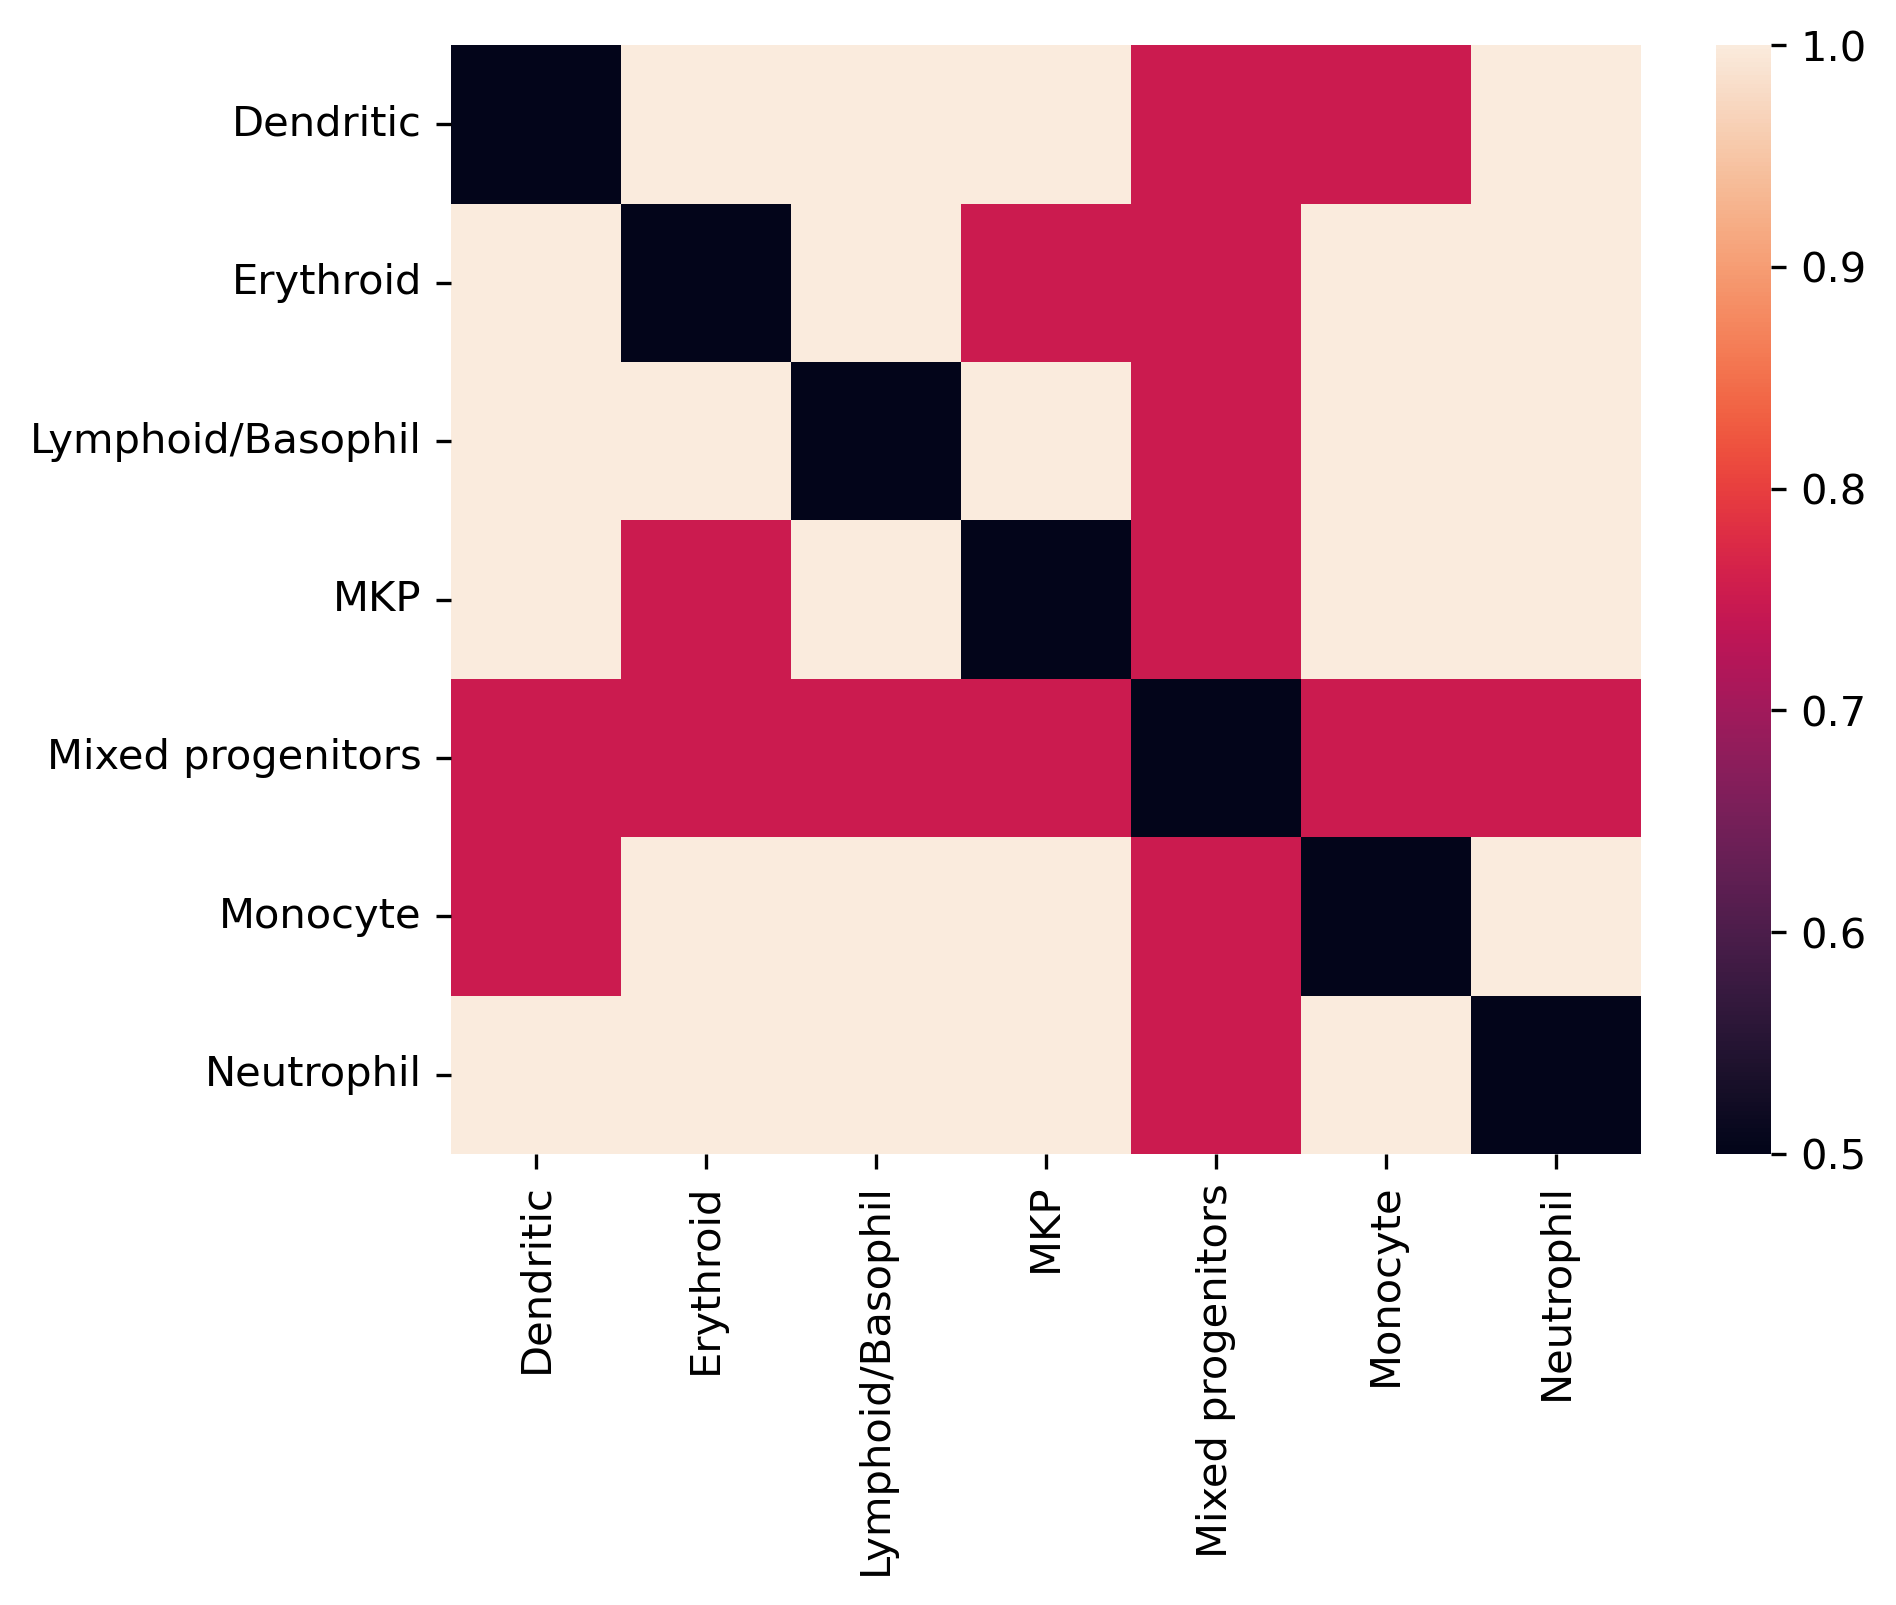
\includegraphics[width=0.5\textwidth]{../figures/hematopoiesis/integration_supervision.png}
  \caption{Supplementary: supervision of OT cost matrix}
\end{figure}

\FloatBarrier
\section{Trajectory inference}

\begin{figure}[!htb]
  \centering
  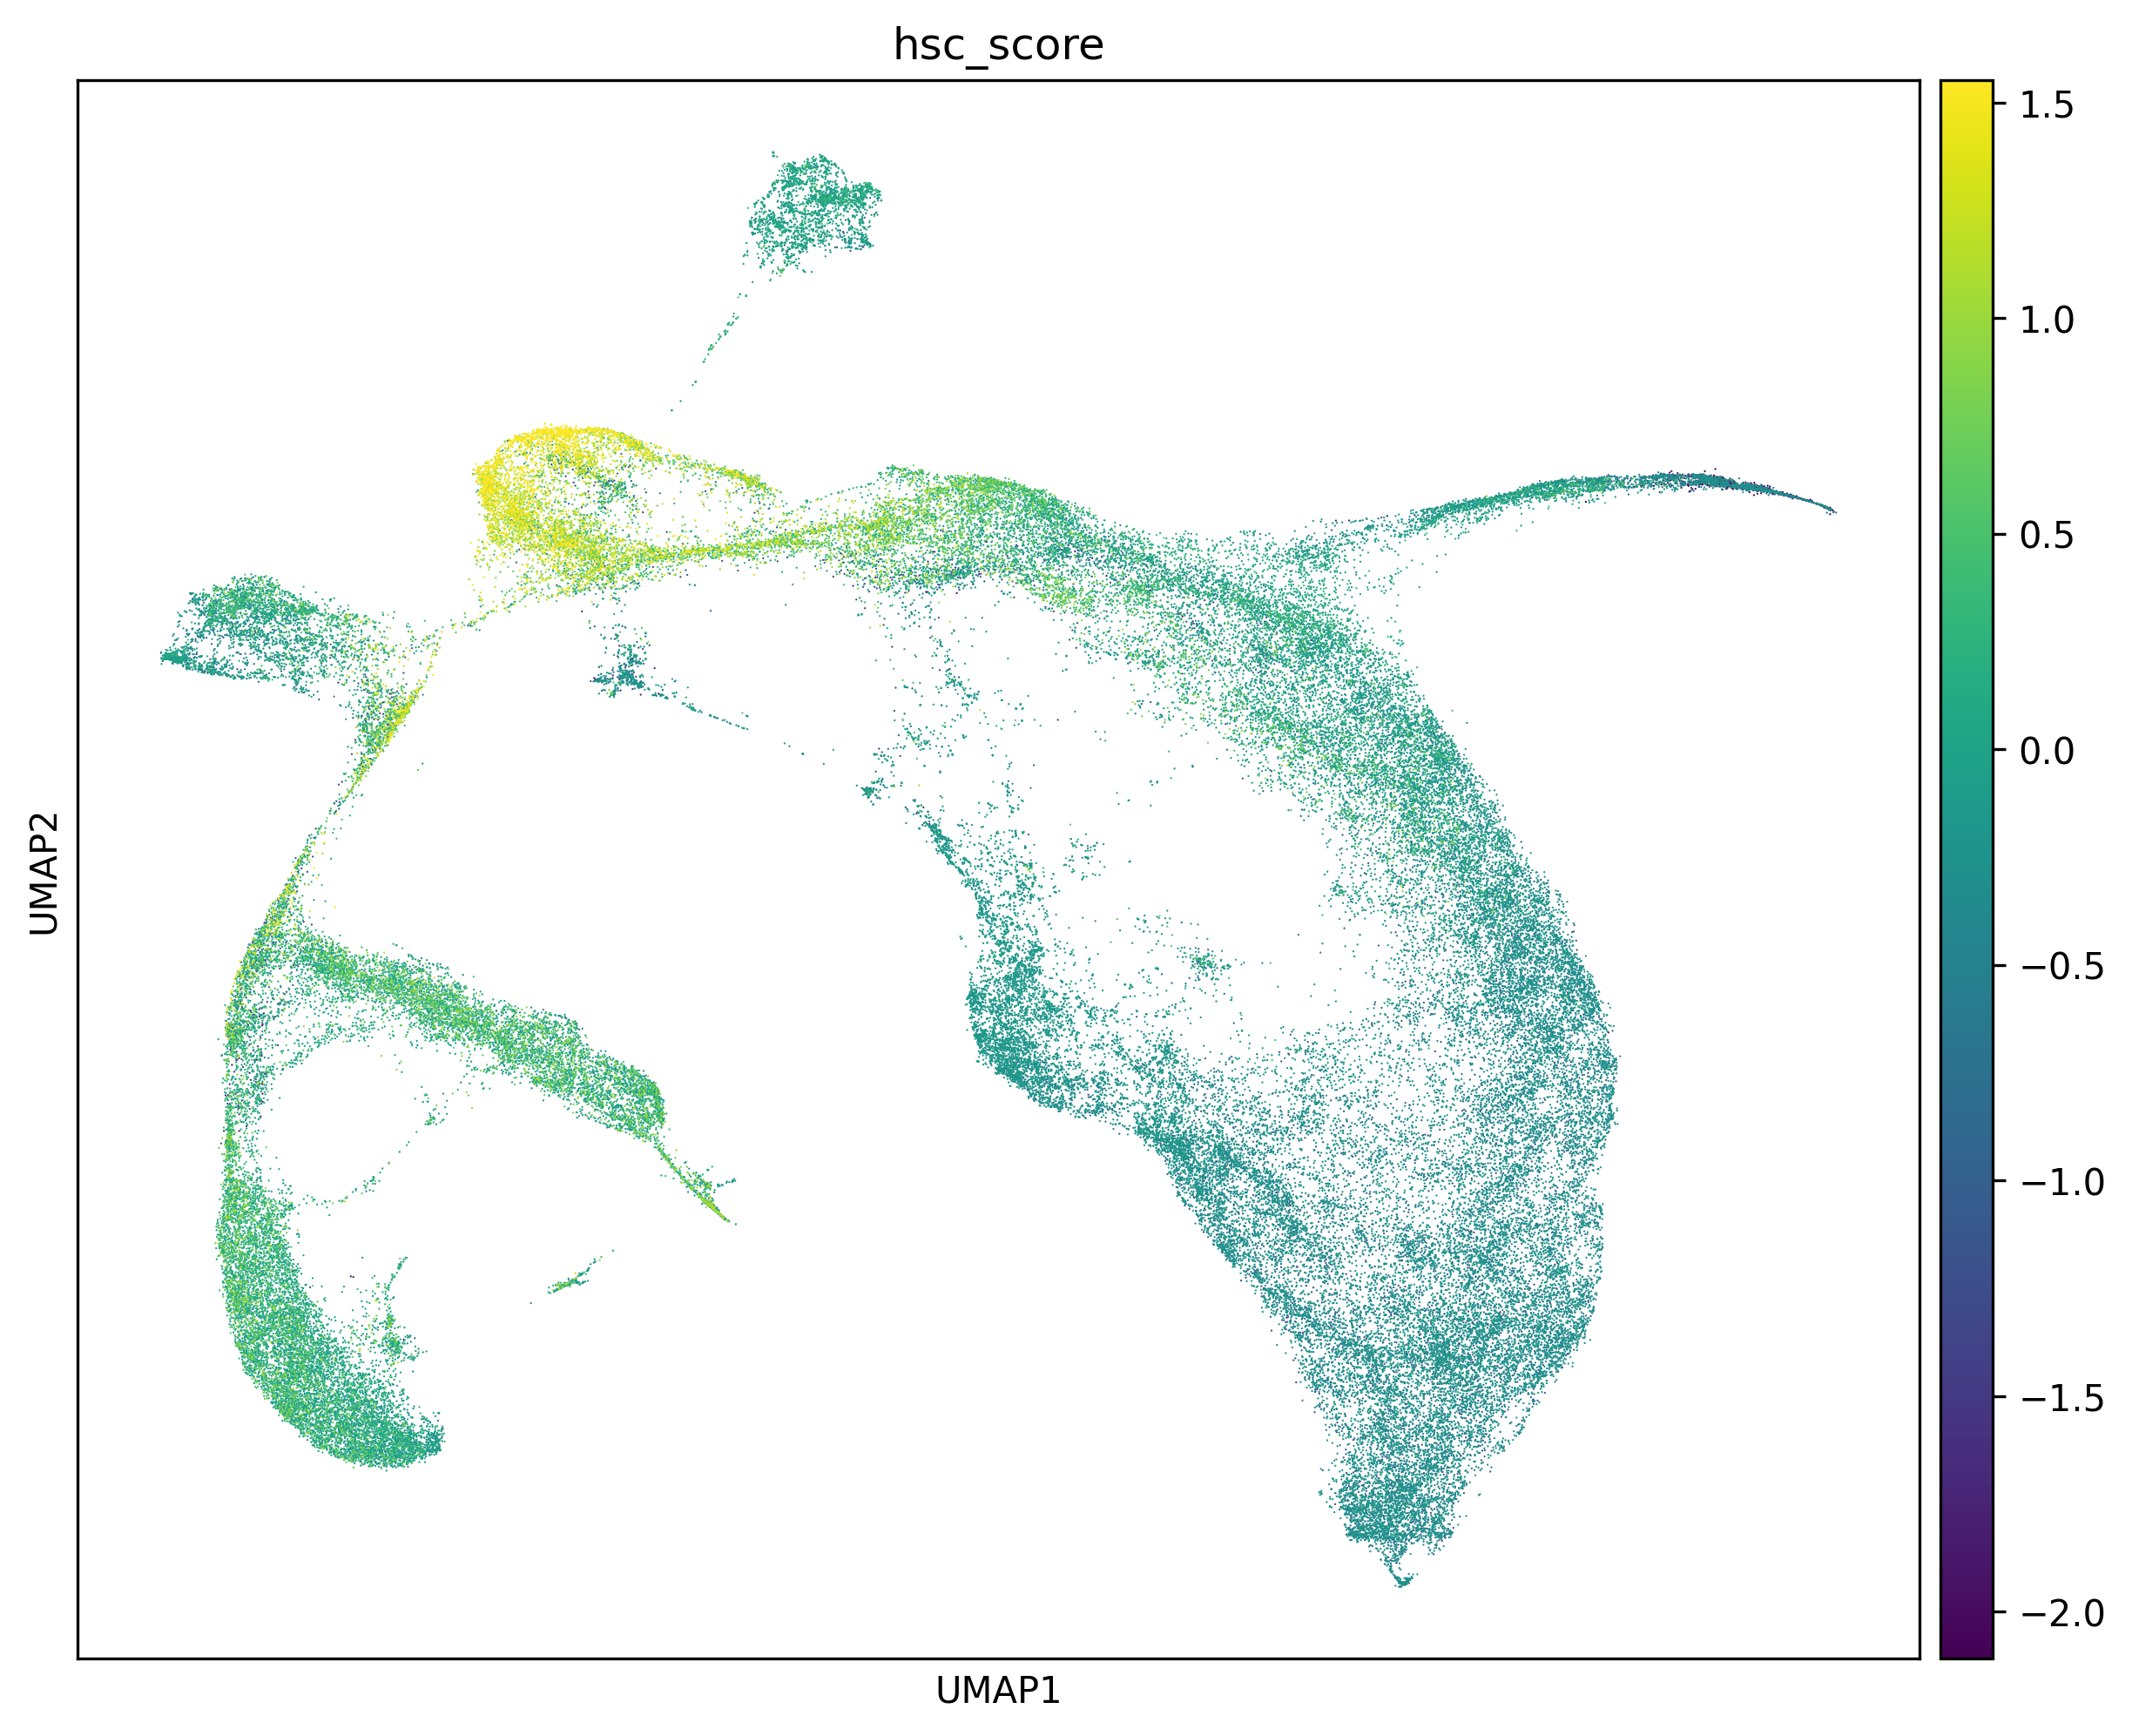
\includegraphics[width=0.5\textwidth]{../figures/hematopoiesis/integrated_hsc_score.png}
  \caption{Supplementary: hematopoeitic stem cell score}
\end{figure}


\end{document}